%%%%%%%%%%%%%%%%%%%%%%%%%%%%%%%%%%%%%%%%%%%%%%%%%%%%%%%%%%%%%%%%%%%%%%%%%%%%%%%
%
% Harvard ALM Thesis
%
% Author: Tony Allen (cyril0allen@gmail.com)
%
%%%%%%%%%%%%%%%%%%%%%%%%%%%%%%%%%%%%%%%%%%%%%%%%%%%%%%%%%%%%%%%%%%%%%%%%%%%%%%%

\documentclass[12pt]{article}
\usepackage[pdftex]{graphicx}
\usepackage{setspace,caption}
\doublespacing


% Default margins are too wide all the way around. I reset them here
\setlength{\topmargin}{1in}
\setlength{\textheight}{7in}
\doublespacing

\begin{document}
\author{Cyril Allen\\
Harvard Extension School}
\renewcommand{\today}{who knows}

%%%%%%%%%%%%%%%%%%%%%%%%%%%%%%%%%%%%%%%%%%%%%%%%%%%%%%%%%%%%%%%%%%%%%%%%%%%%%%%

\tableofcontents
\listoffigures

%%%%%%%%%%%%%%%%%%%%%%%%%%%%%%%%%%%%%%%%%%%%%%%%%%%%%%%%%%%%%%%%%%%%%%%%%%%%%%%
\section{Abstract}

% TODO

%%%%%%%%%%%%%%%%%%%%%%%%%%%%%%%%%%%%%%%%%%%%%%%%%%%%%%%%%%%%%%%%%%%%%%%%%%%%%%%
\section{Introduction}

With the advent of cloud computing, datacenters are making use of distributed
applications more than ever. Companies like Google use software such as
MapReduce to generate over 20 petabytes of data per day using very large
numbers of commodity servers [3]. Many other companies use large scale clusters
to perform various computational tasks via the the open-source MapReduce
implementation, Hadoop [4], or they can possess a virtualized datacenter
allowing them to migrate virtual machines between various machines for
high-availability reasons. As economics change for hardware, it is likely that
a scalable cloud will have the requirement to mix node types, which will lead
to higher performance/capacity nodes being mixed with lower
performance/capacity HDD nodes. This thesis presents an adaptive data placement
method in the Nutanix distributed file system (ADSF) which will attempt to
remedy the common problems found in many heterogeneous clustered file systems.

  \subsection{Motivation}

  A number of scenarios arise in heterogeneous Nutanix clusters that can
  degrade performance for an entire cluster. The currently replica disk
  selection logic in Stargate uses does not take into account a number of
  variables such as disparities in tier size, CPU power, workloads, and disk
  health among other things.

  Considering that a write is not complete until all replicas are written, the
  write's performance is at the mercy of the slowest disk and node.  There are
  several scenarios, both pathological and daily occurences, where a more
  robust replica placement heuristic is required. For the work in this thesis,
  I will focus on two orthogonal cases described below.

    \subsubsection{Interfering Workloads}

    An example of interfering workloads can take the form of a 3-node
    homogeneous cluster with only 2 nodes hosting active workloads as shown in
    Figure \ref{fig:workload_disparity}. In the current random selection scheme
    in use by the ADSF, writes are equally likely to place their replica on the
    other node with an active workload as they would be to place it on the idle
    node. This can impact performance on both the local and remote workloads as
    secondary writes will be slower on nodes whose resources are being utilized
    by their primary workloads. An adaptive replica placement scheme is needed
    to avoid the busy node and bias secondary replica placement on an idle
    node. 

    \begin{figure}[h]
      \centering
      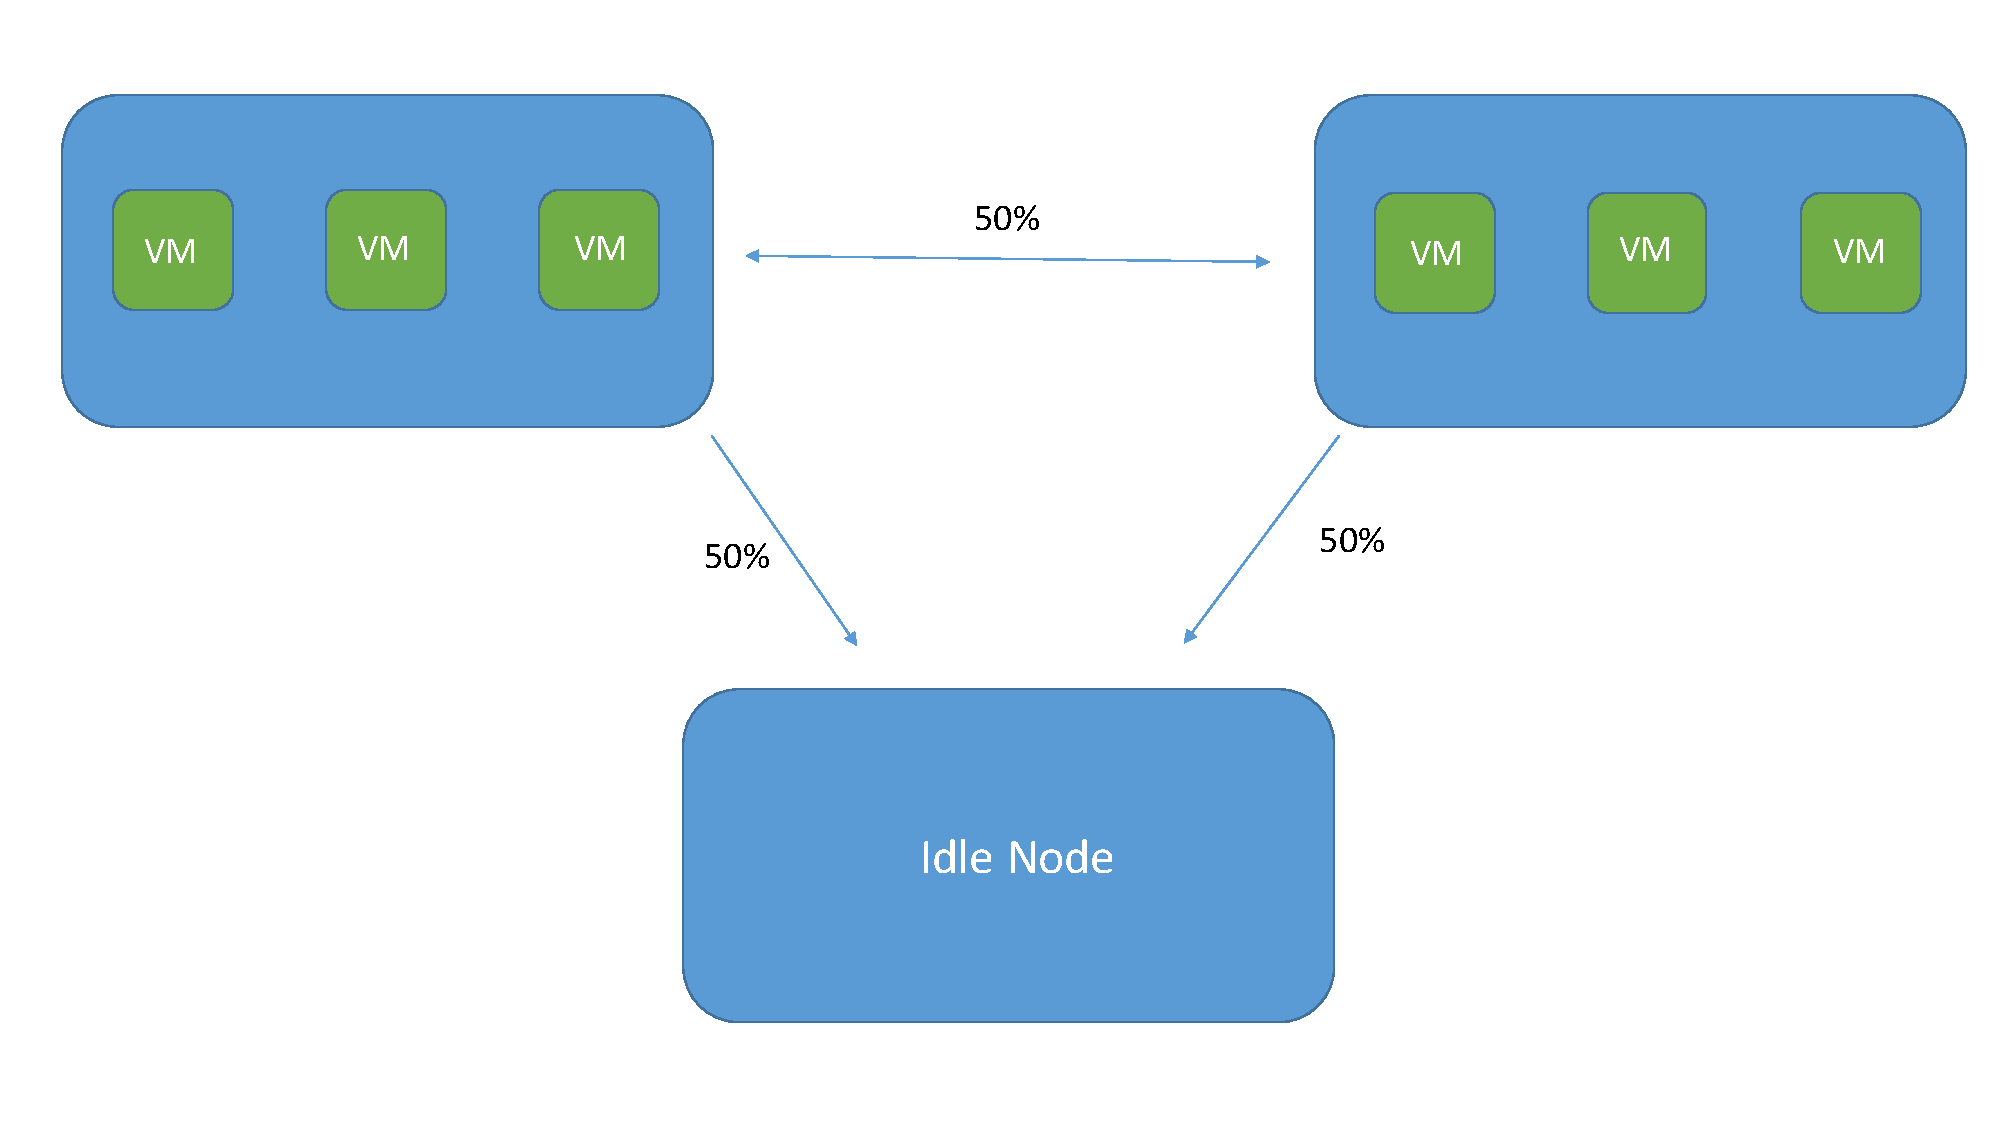
\includegraphics[scale=0.4]{images/homogeneous_workload_disparity.pdf} 
      \caption{A cluster with identical nodes running a heterogeneous workload.}
      \label{fig:workload_disparity}
    \end{figure}

    \subsubsection{Nodes with Tier Size Disparities}

    A cluster containing nodes with a tier size disparity are susceptible to a
    skew in node fullness, even if the workload on each node is identical. This
    can be illustrated via Figure \ref{fig:tier_size_disparity} where we have a
    3-node heterogeneous cluster with 2 high-end nodes and a single weak node.
    Suppose these high-end nodes have 500GB of SSD tier and 6TB of HDD tier and
    the single weak node has only 128GB of SSD tier and 1TB of HDD tier. If 3
    simultaneous workloads were to generate data such that the working sets of
    the workloads are 50\% of the local SSD tier, the weaker node is at a
    significant disadvantage. Given the current NDFS replica selection
    algorithm, we can expect 500GB of replica traffic to flood the weak node
    and fill up its SSD tier well before the workload is finished. This results
    in an inability for the workload on the smaller node to place its primary
    replicas locally and forces the workload to rely on remote CVMs, increasing
    latency. An adaptive replica placement heuristic would mitigate this issue
    by taking disk usages into consideration during the placement of secondary
    replicas and biasing placement of secondary replicas on the nodes with more
    free capacity.

    \begin{figure}[h]
      \centering
      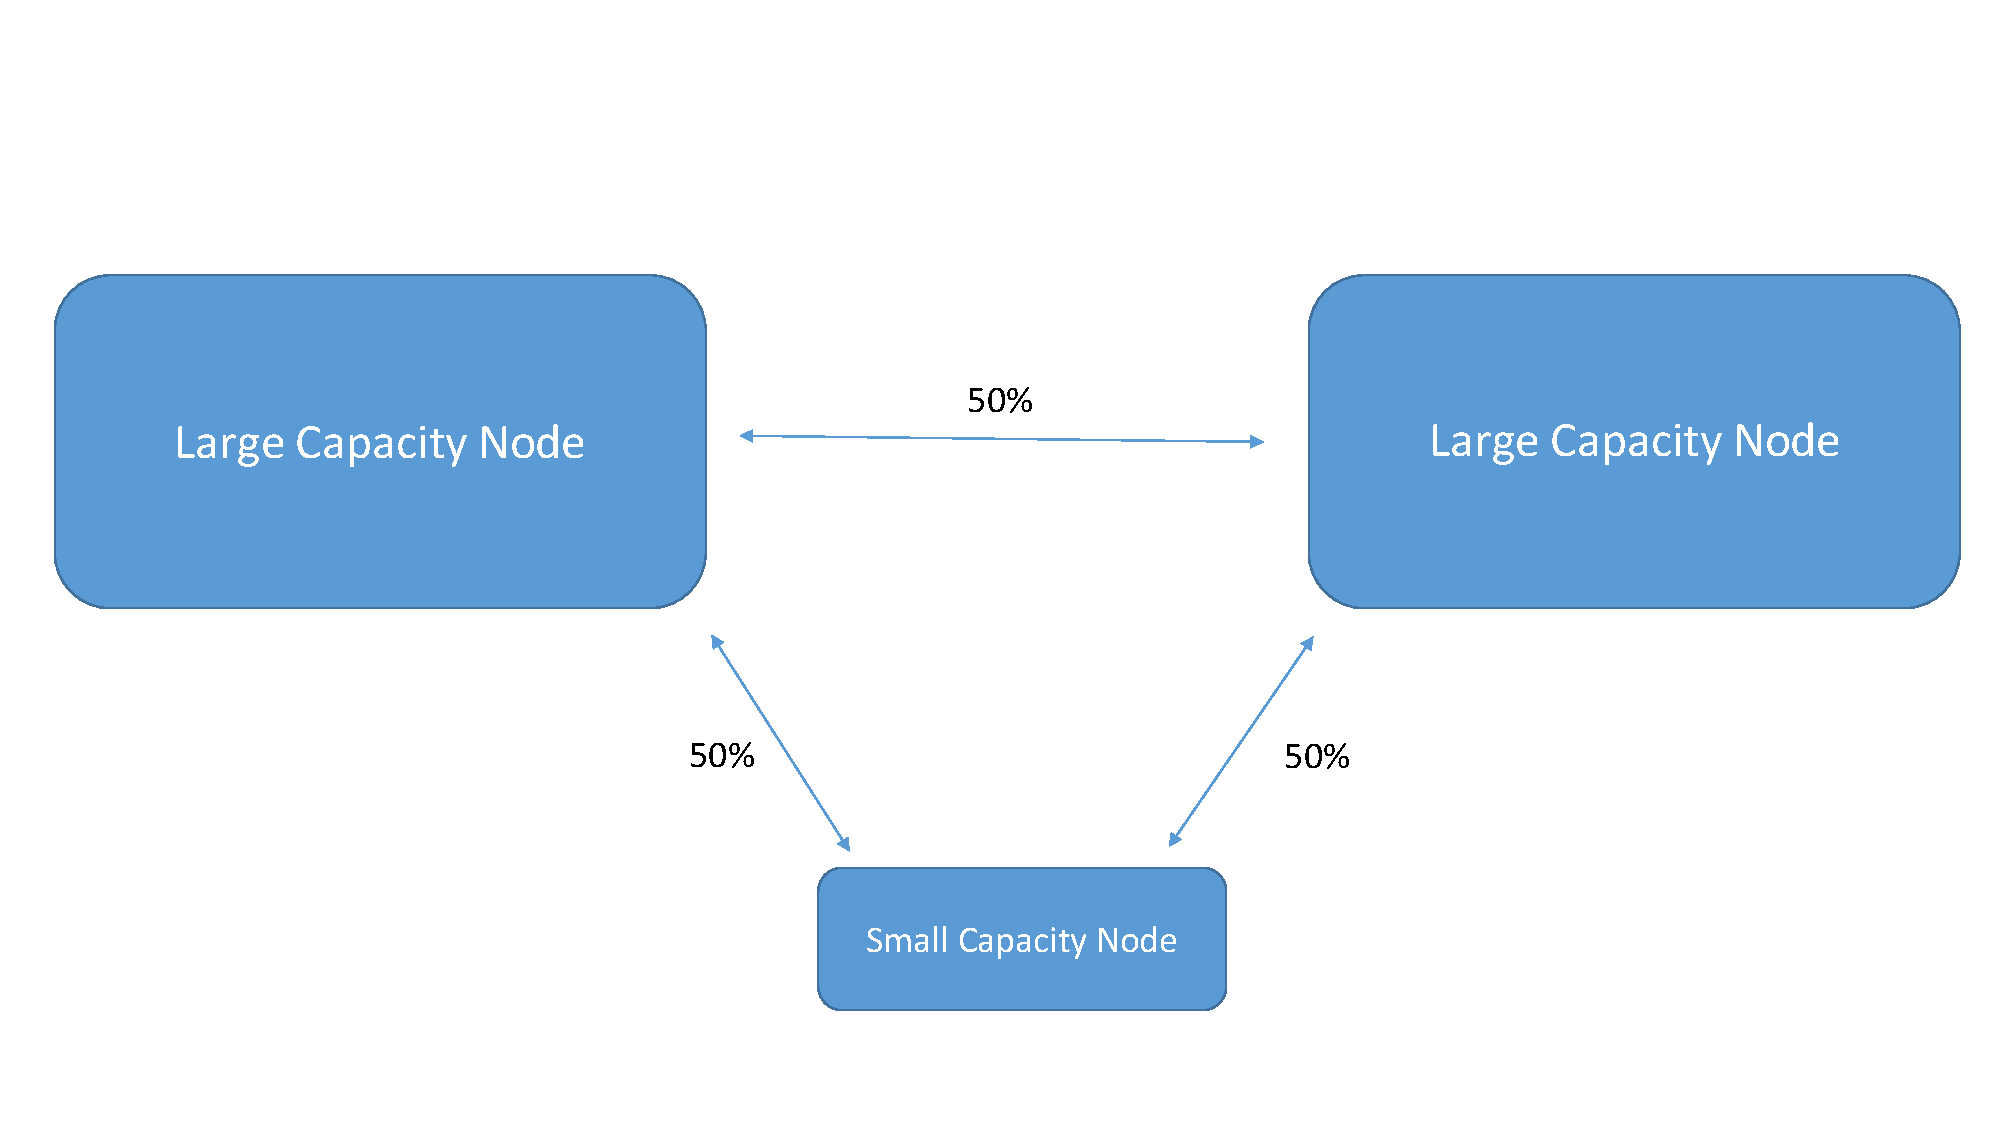
\includegraphics[scale=0.4]{images/homogeneous_tier_disparity.pdf} 
      \caption{A cluster with nodes of varying resource capacity.}
      \label{fig:tier_size_disparity}
    \end{figure}

  \subsection{Acropolis Base System}

  NDFS is facilitated by a clustering of controller virtual machines (CVMs)
  which reside, one per node, on each server in the cluster. The CVM presents
  via NFS (for VMWare's ESXi [14]), SMB (for Microsoft's Hyper-V [17]), or
  iSCSI (for Nutanix's AHV [1]) an interface to each hypervisor that they
  reside on. For example, the interface provided by the CVMs to VMware's ESXi
  hypervisor [14] will be interfaced with as a datastore. The virtual machines'
  virtual disk files will reside on the Nutanix datastore and be accessed via
  NFS through the CVM sharing a host with the user VM. Within the CVM exists an
  ecosystem of process that make up the ADSF. This work is scoped specifically
  to the I/O manager process, Stargate.


  \subsection{Stargate}

  The Stargate process is responsible for all data management and I/O
  operations. The NFS/SMB/iSCSI interface presented to the hypervisor is also
  presented by Stargate. All file allocations and data replica placement
  decisions are made by this process.

  As the Stargate process facilitates writes to physical disks, it gathers
  statistics for each disk such as the number of operations currently in flight
  on the disk (queue length), how much data in bytes currently resides on the
  disk, and average time to complete an operation on the disk. These statistics
  are only gathered on the local disks; however, they are then stored in a
  distributed database provided by another ADSF service along with the
  statistics gathered by every other Stargate in the cluster. These disk
  statistics stored in the database and are pulled periodically and are then
  used to make decisions on data placement when performing writes.

    \subsubsection{Oplog and Extent Store}

% TODO

    \subsubsection{Storage Tiering}

% TODO

    \subsubsection{Data Replication and Fault Tolerance}

% TODO

    \subsubsection{Replica Selection}

% TODO

%%%%%%%%%%%%%%%%%%%%%%%%%%%%%%%%%%%%%%%%%%%%%%%%%%%%%%%%%%%%%%%%%%%%%%%%%%%%%%%
\section{Prior Work}

% TODO

%%%%%%%%%%%%%%%%%%%%%%%%%%%%%%%%%%%%%%%%%%%%%%%%%%%%%%%%%%%%%%%%%%%%%%%%%%%%%%%
\section{Implementation}

% TODO

  \subsection{Overview}

% TODO

  \subsection{Fitness Values and Functions}

% TODO

  \subsection{Weighted Random Selection Algorithms}

  After a weight is calculated for a disk in the cluster that will store a
  replica, the WeightedVector class' Sample() calls will perform a weighted
  random selection on the set of potential candidate disks. To determine the
  best method of weighted random selection for Stargate's WeightedVector class,
  an exploration of various weighted random selection algorithms was necessary.
  Since the file system only supports replication factors of 2 or 3, the
  investigation was limited to algorithms that allow for a weighted $N$ choose
  $Y$, where $Y$ is the data replication factor.

  %TODO: Talk about herding here.
  
  This section provides an overview of the algorithms investigated via
  simulations to compare each algorithm at different orders of magnitude.

    \subsubsection{Scalability Simulation Methodology}
     To test the scalability of the weighted random selection algorithms
     evaluated in the next section, a single-threaded Python script was written
     to to evaluate the change in run time as sample sets increase. Each
     algorithm's time to select is calculated for each of a fixed number of
     iterations for multiple sample sets. pseudo-code for the simulations
     can be written as follows:

     \begin{verbatim}
     for each selection_algorithm in algorithm_list:
         run_time_values = empty_list()
         for each sample_set_size in all_sample_set_sizes:
             sample_set = generate_sample_set(sample_set_size)
             all_elapsed_times = empty_list()
             for each iteration:
                 start_time = time.now()
                 selection_algorithm(sample_set)
                 elapsed_time = time.now() - start_time
                 all_elapsed_times.append(elapsed_time)
             calculate_avg_elapsed_time(all_elapsed_times)
             calculate_std_error(all_elapsed_times)
     \end{verbatim}
        
    Object weights are constant throughout the simulation, so selection schemes
    that require some amount of preprocessing (such as the top T\% calculation
    for truncation selection) are performing their preprocessing steps for each
    selection. This gives information about the worst-case behavior for each
    algorithm in comparison with others'.

    \subsubsection{Herding Behavior Evaluation Methodology}
    Herding behaviors can be seen in some weighted random selection
    algorithms when (TODO: cite some papers) the weights of a subset of objects
    in the sampling pool cause a disproportionate amount of selections to
    target those objects. In the case of replica disk selections in a Nutanix
    cluster, this can cause too many operations to target an especially
    suitable disk, resulting in poor performance. We can simulate an
    exaggerated scenario in which the susceptibility to herding behavior can be
    observed by having a single object with a weight that is multiple orders of
    magnitude heavier than the next highest object in the sampling set. It is
    also necessary to observe any herding behavior for a sampling set with low
    weight skew. This section describes the simulation methodology for each.

    High-skew sampling sets of 11 objects were generated such that the array
    index of the first 10 objects was assigned as the object weight, and the
    last object was given a weight of 1000. This creates an extremely large
    skew in weights and makes the high-weight object a target for herding
    behavior. Given this sampling set, weighted random selections were
    performed and a histogram was kept that tracked the number of selections
    for each object. 1e3, 1e4, and 1e5 iterations were performed to observe any
    changes in herding behavior at larger time scales. In addition to the
    high-skew sampling sets, low-skew sets of 100 objects were also simulated.
    These low-skew sets were identical to the high-skew sets, except there was
    not a single object with an exaggerated weight of 1000. All element weights
    were their array indices.

    \subsubsection{Stochastic Universal Sampling (SUS) Simulations}
    SUS is another sampling technique first introduced by Baker in 1987 [10].
    The algorithm can be understood as follows: On a standard roulette wheel
    there's a single pointer that indicates the winner. The roulette wheel's
    "bins" can all be the same size which would indicate a uniform probability
    of selecting any bin and could also be unevenly sized which would indicate
    a weighted probability. SUS uses this same concept except allows for N
    evenly spaced pointers corresponding to the selection of N items. Key
    things to note are that the set, or "bins" in my roulette analogy, must be
    shuffled prior to selection. Also, there is a minimum spacing allowed for
    the pointers to prevent selection of the same bin.

    \begin{figure}[h]
      \centering
      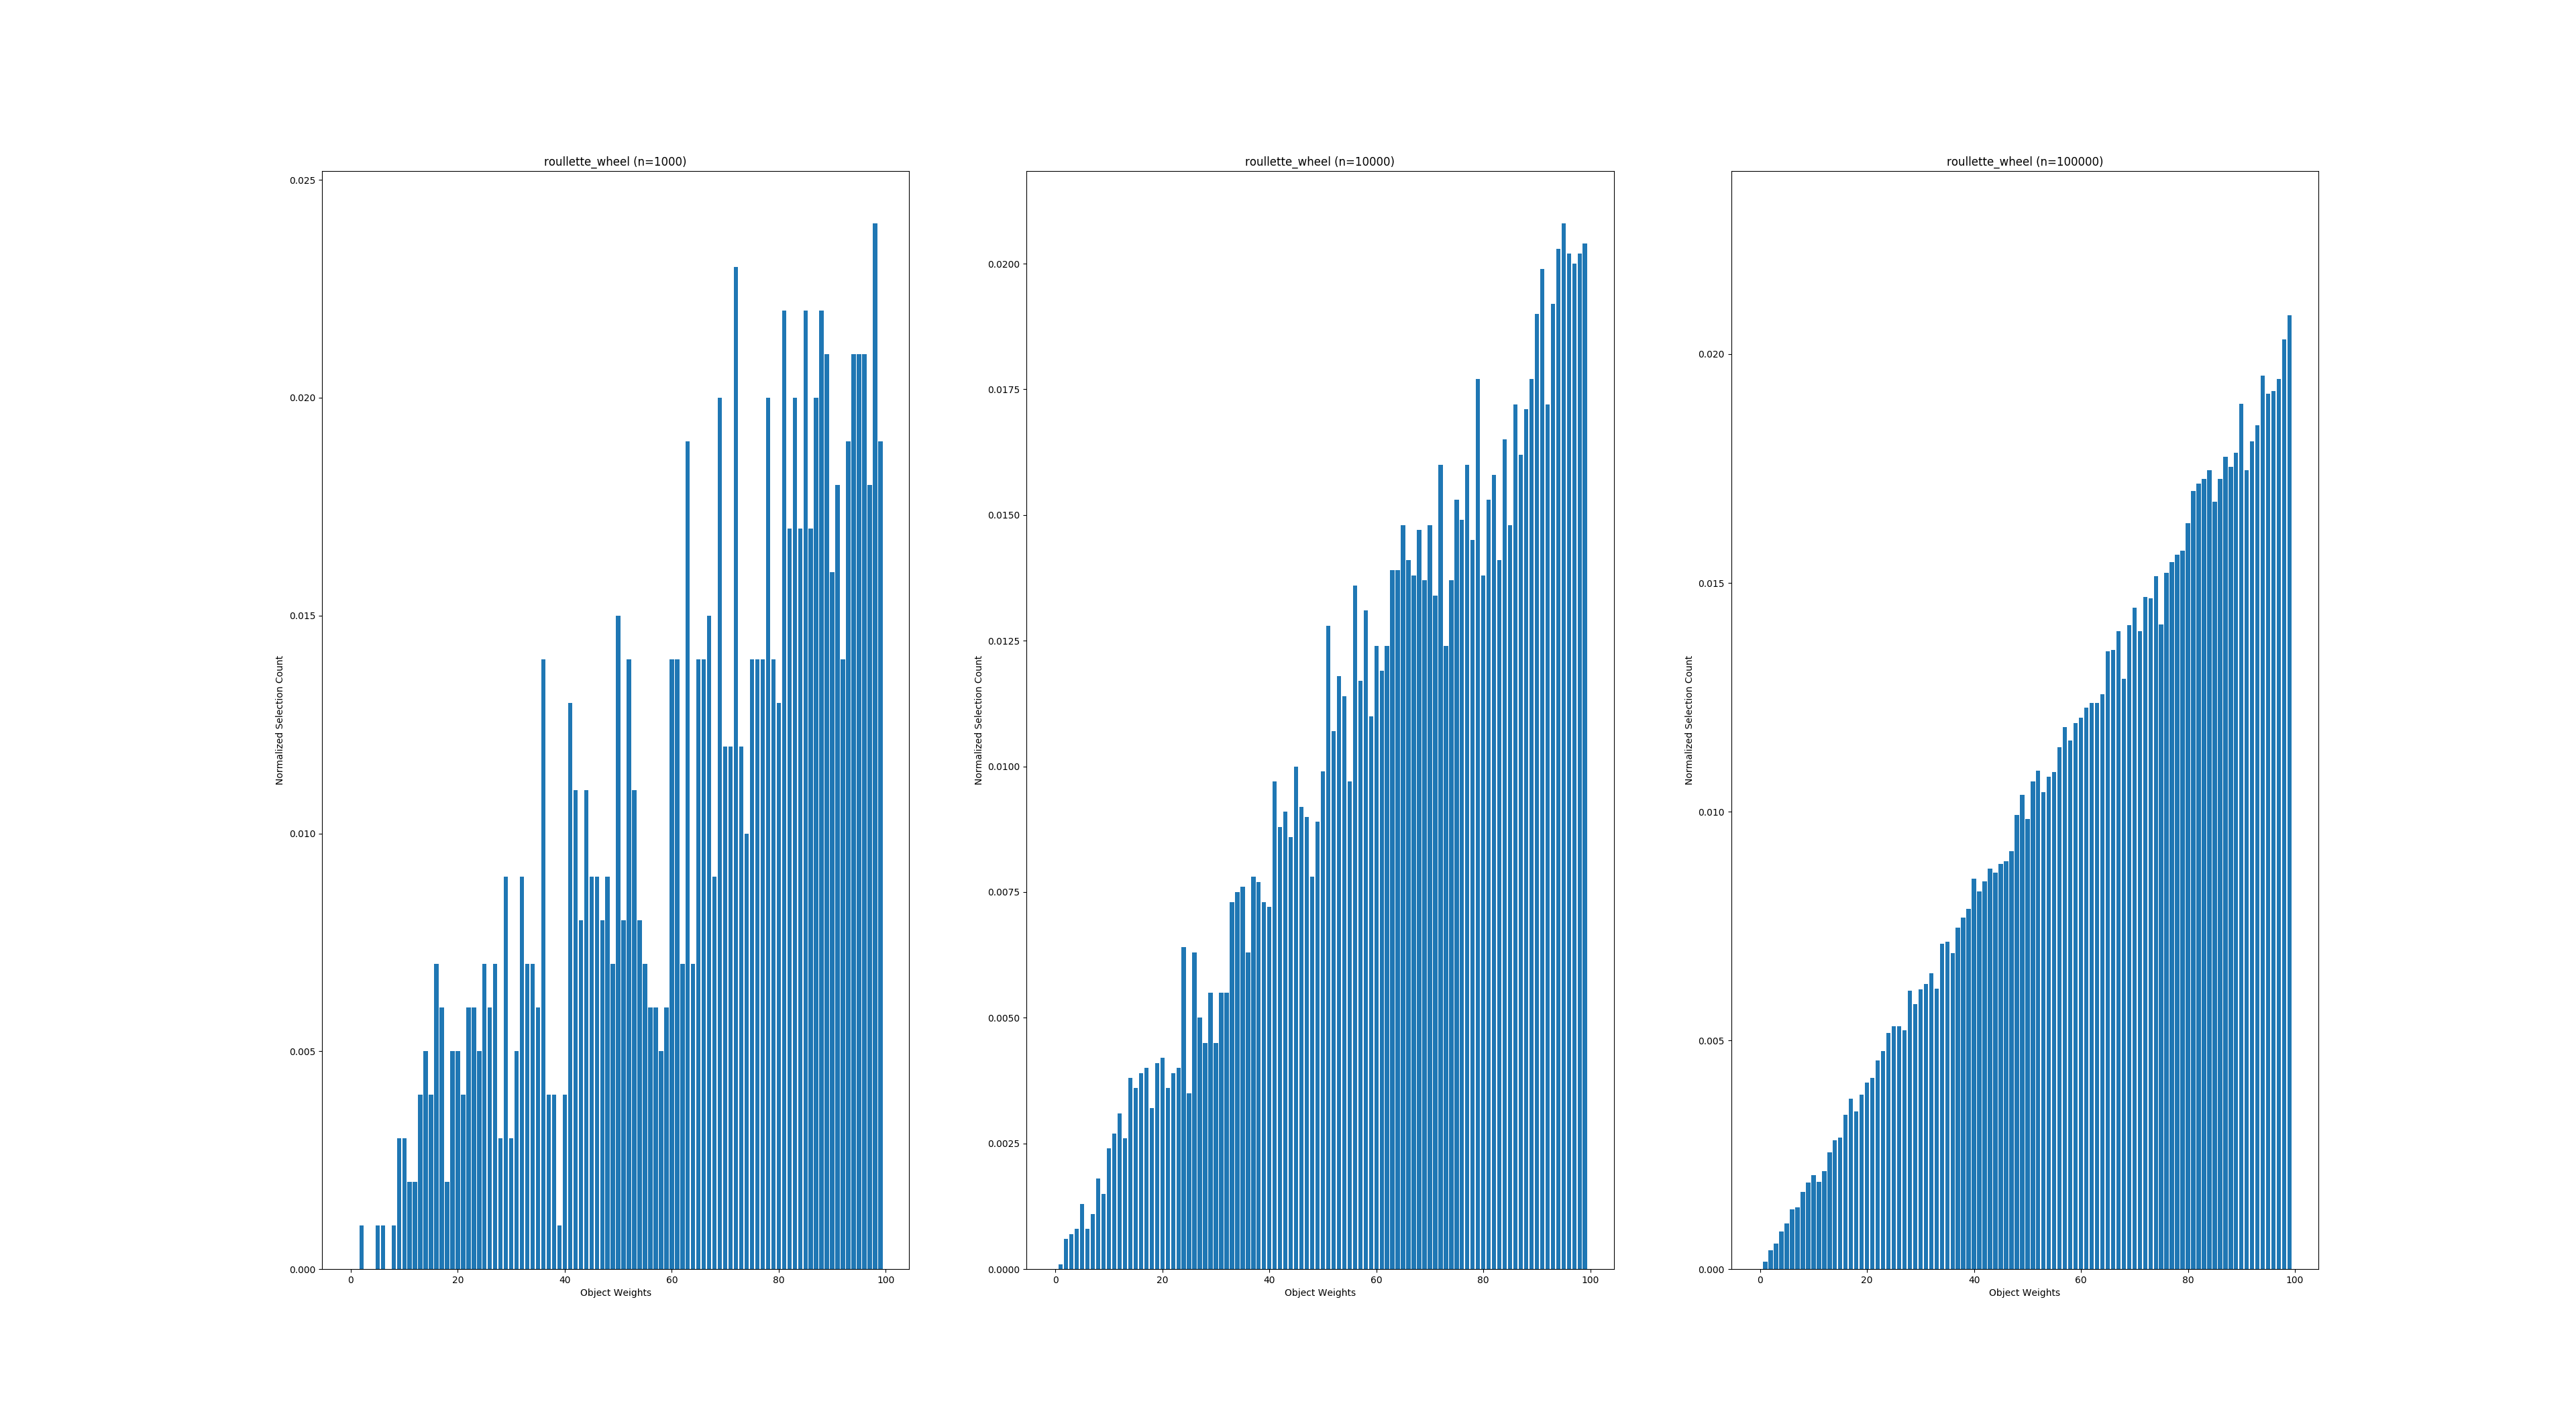
\includegraphics[scale=0.30]{images/herding_roullette.png} 
      \caption{Histograms generated by simulation of Stochastic Universal
               Sampling using sample sizes of 1e3, 1e4, and 1e5. Object weights
               for the histograms are in the range [1,100].}
      \label{fig:herding_roullette}
    \end{figure}

    \begin{figure}[h]
      \centering
      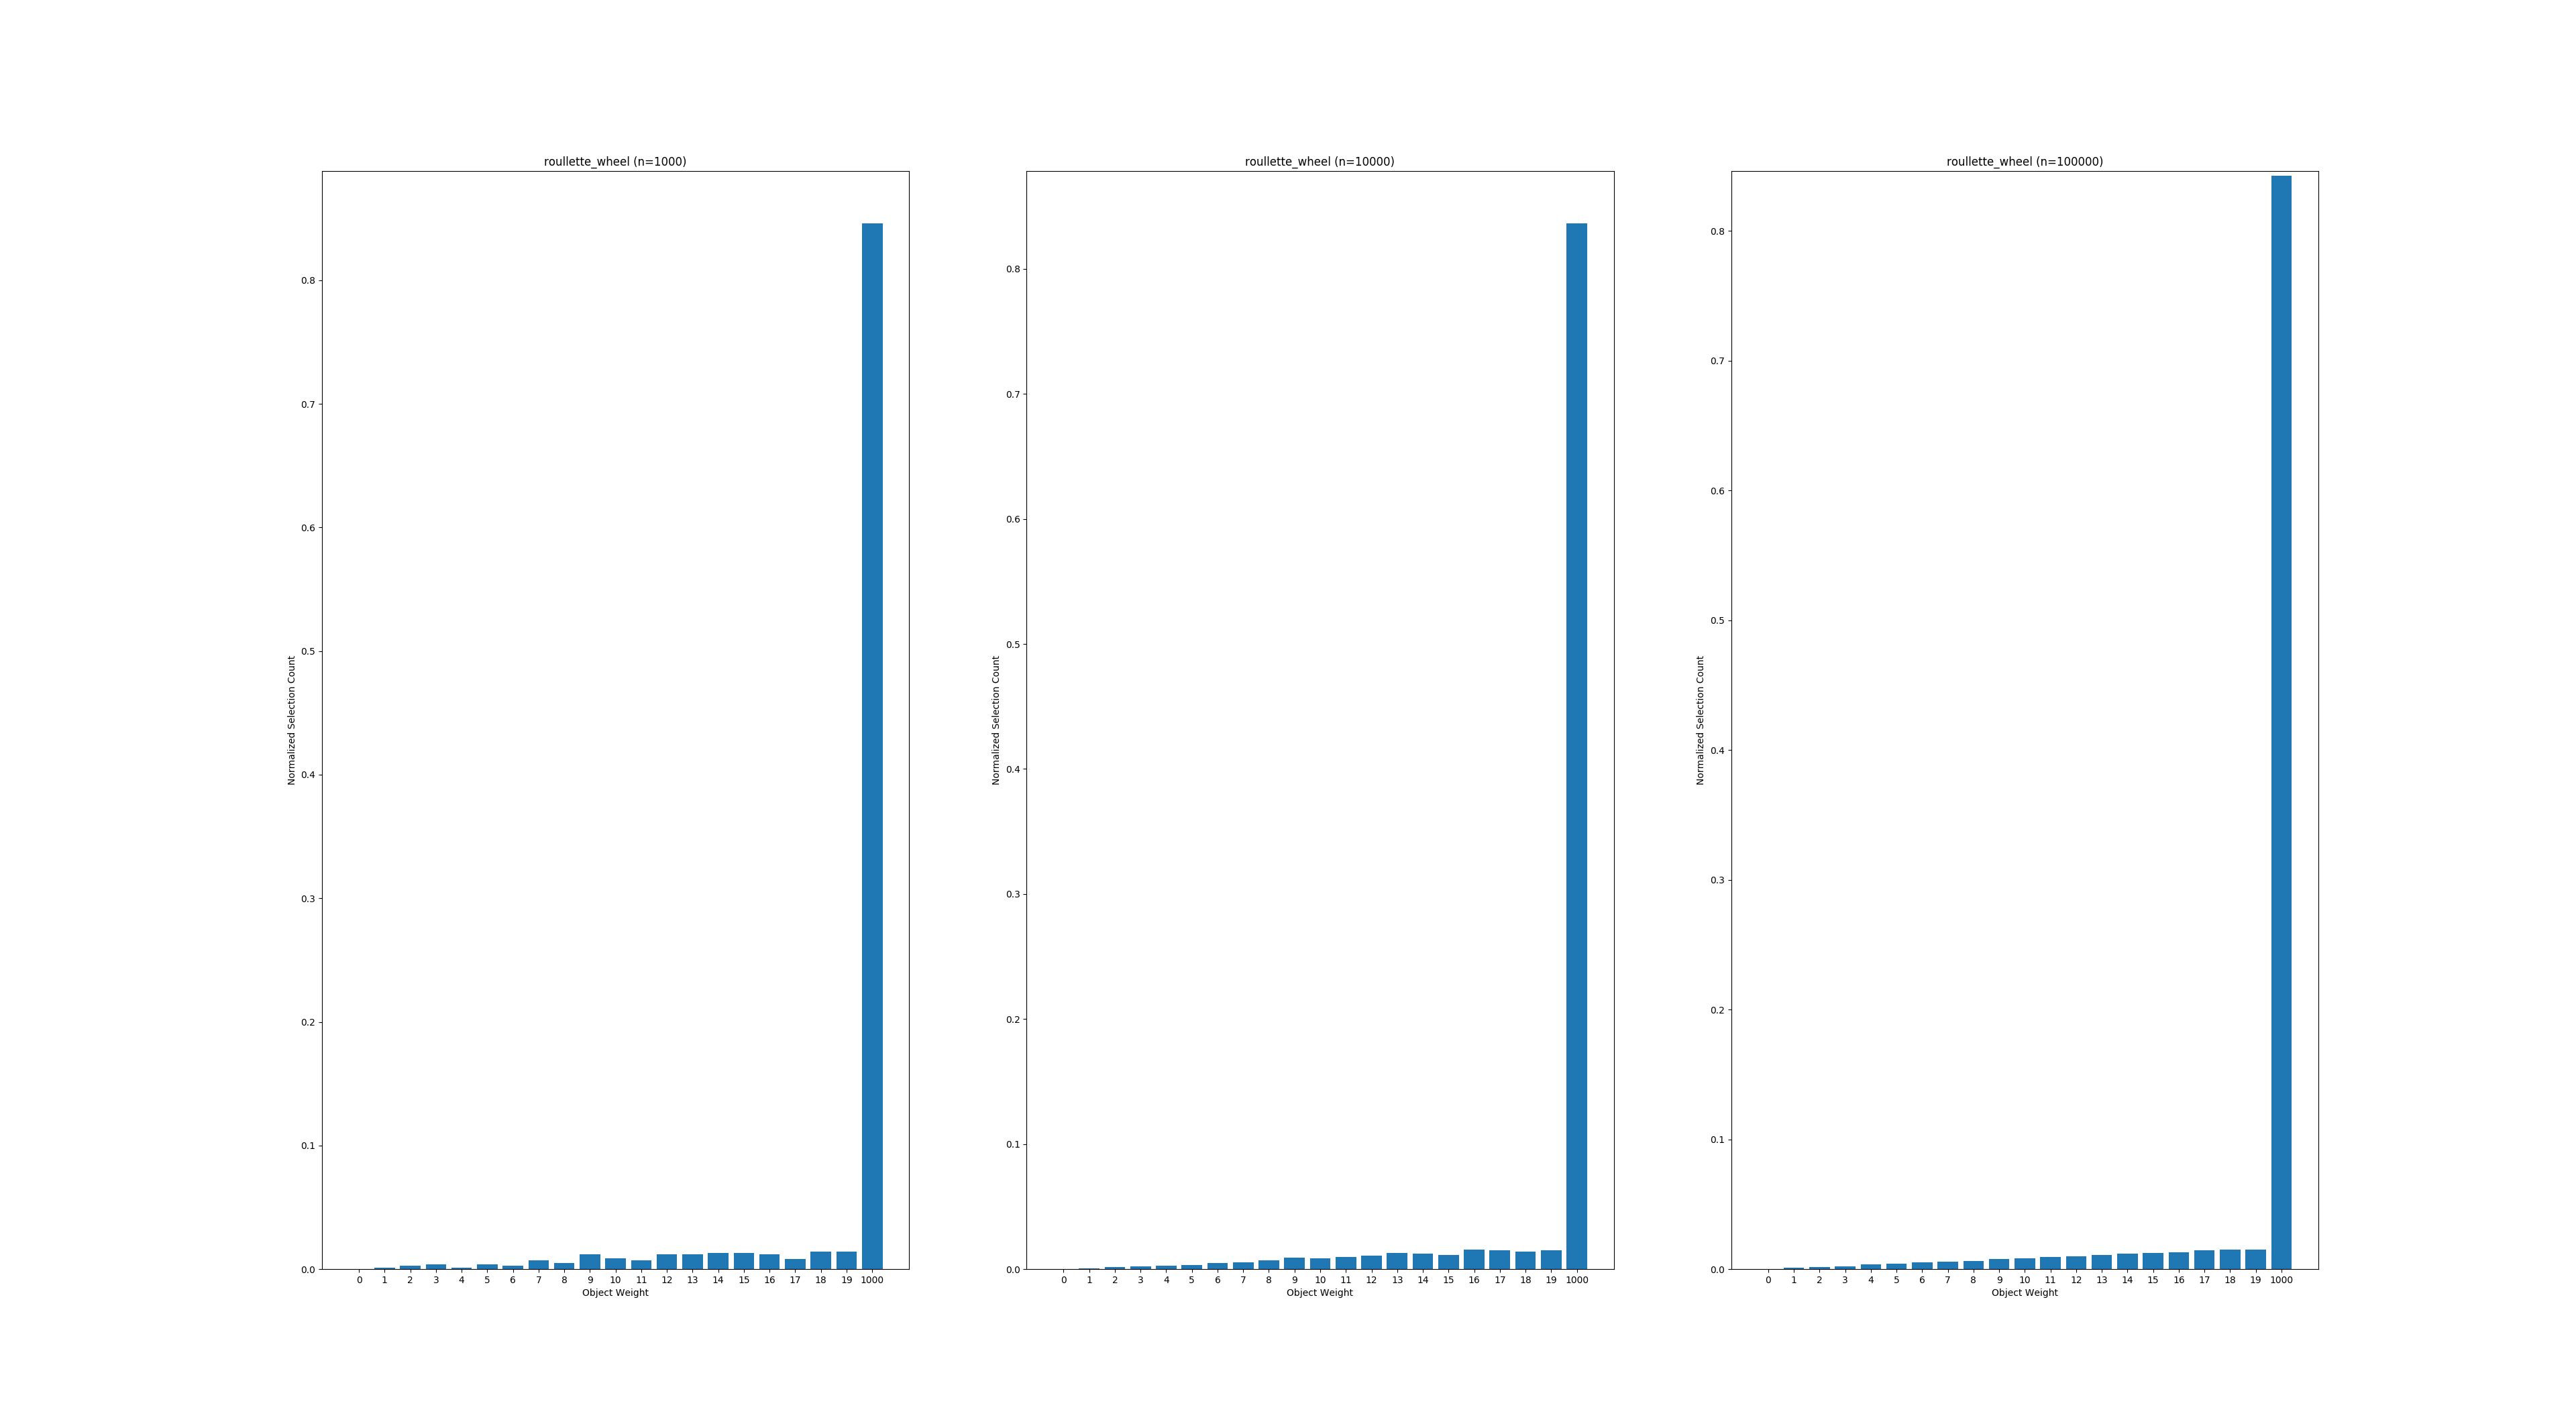
\includegraphics[scale=0.30]{images/pathological_roullette.png} 
      \caption{Histograms generated by simulation of Stochastic Universal
               Sampling using sample sizes of 1e3, 1e4, and 1e5. Object weights
               are in the range [0,9] with a single outlier of weight 1000 to
               illustrate the effect of herding behavior.}
      \label{fig:pathological_roullette}
    \end{figure}

    Figure \ref{fig:herding_roullette} shows the evolution of the
    distribution of selection frequencies for SUS as the number of samples
    increases. We can see that the selection frequency is proportional to the
    object weight. This can prove problematic for outlier objects with weights
    that are much larger than the other objects in the set as shown in Figure
    \ref{fig:pathological_roullette}. We can see that the high weight object's
    selection frequency eclipses all other objects in the selection pool which
    can lead to extreme herding behaviors.

    \subsubsection{Tructation Selection Simulations}
    Truncation selection[TODO: CITE] does not consider any objects for
    selection below some threshold, $T$. In figure
    \ref{fig:herding_truncation}, only the top 10\% of objects ranked by weight
    are considered for selection. Within this subset, weight has no meaning so
    there is a uniform distribution of selections. However, this may not be
    suitable for use cases where all objects must be candidates for selection.
    Depending on the threshold chosen, this algorithm can be resistant to
    herding behavior as shown in Figure \ref{fig:pathological_truncation}. 

    \begin{figure}[h]
      \centering
      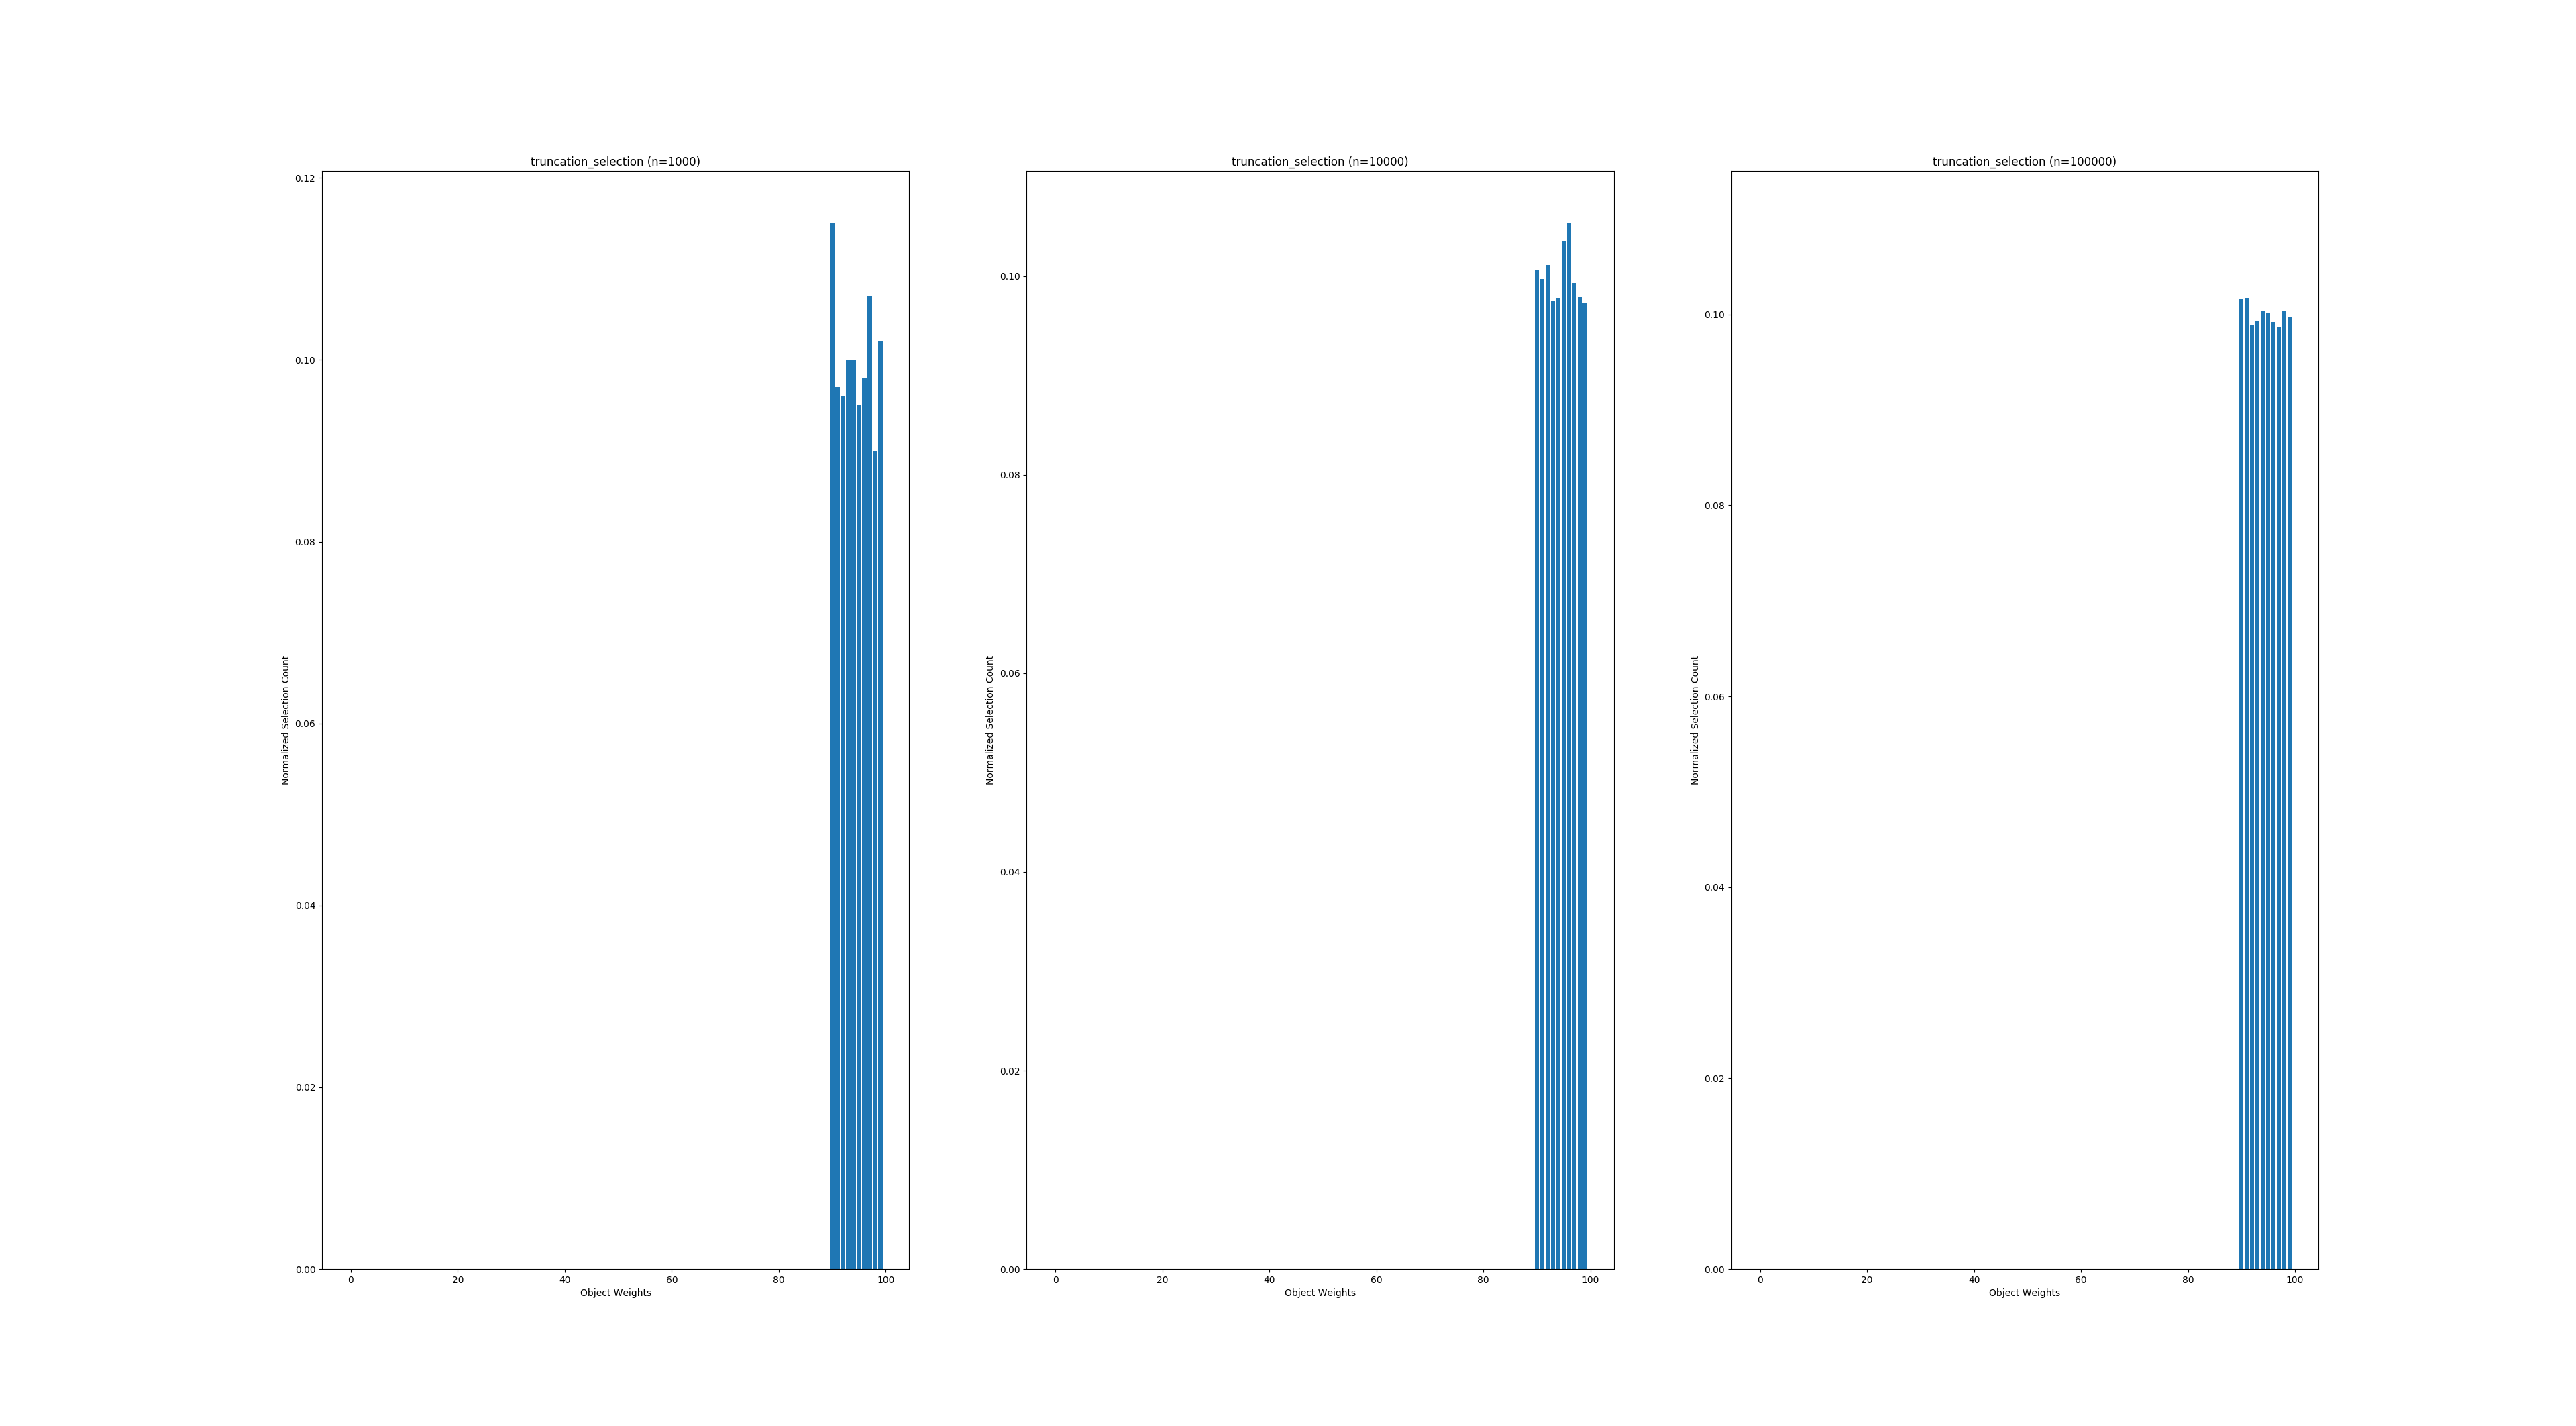
\includegraphics[scale=0.30]{images/herding_truncation.png} 
      \caption{Histograms generated by simulation of truncation selection
               using sample sizes of 1e3, 1e4, and 1e5. Object weights
               for the histograms are in the range [1,100].}
      \label{fig:herding_truncation}
    \end{figure}

    \begin{figure}[h]
      \centering
      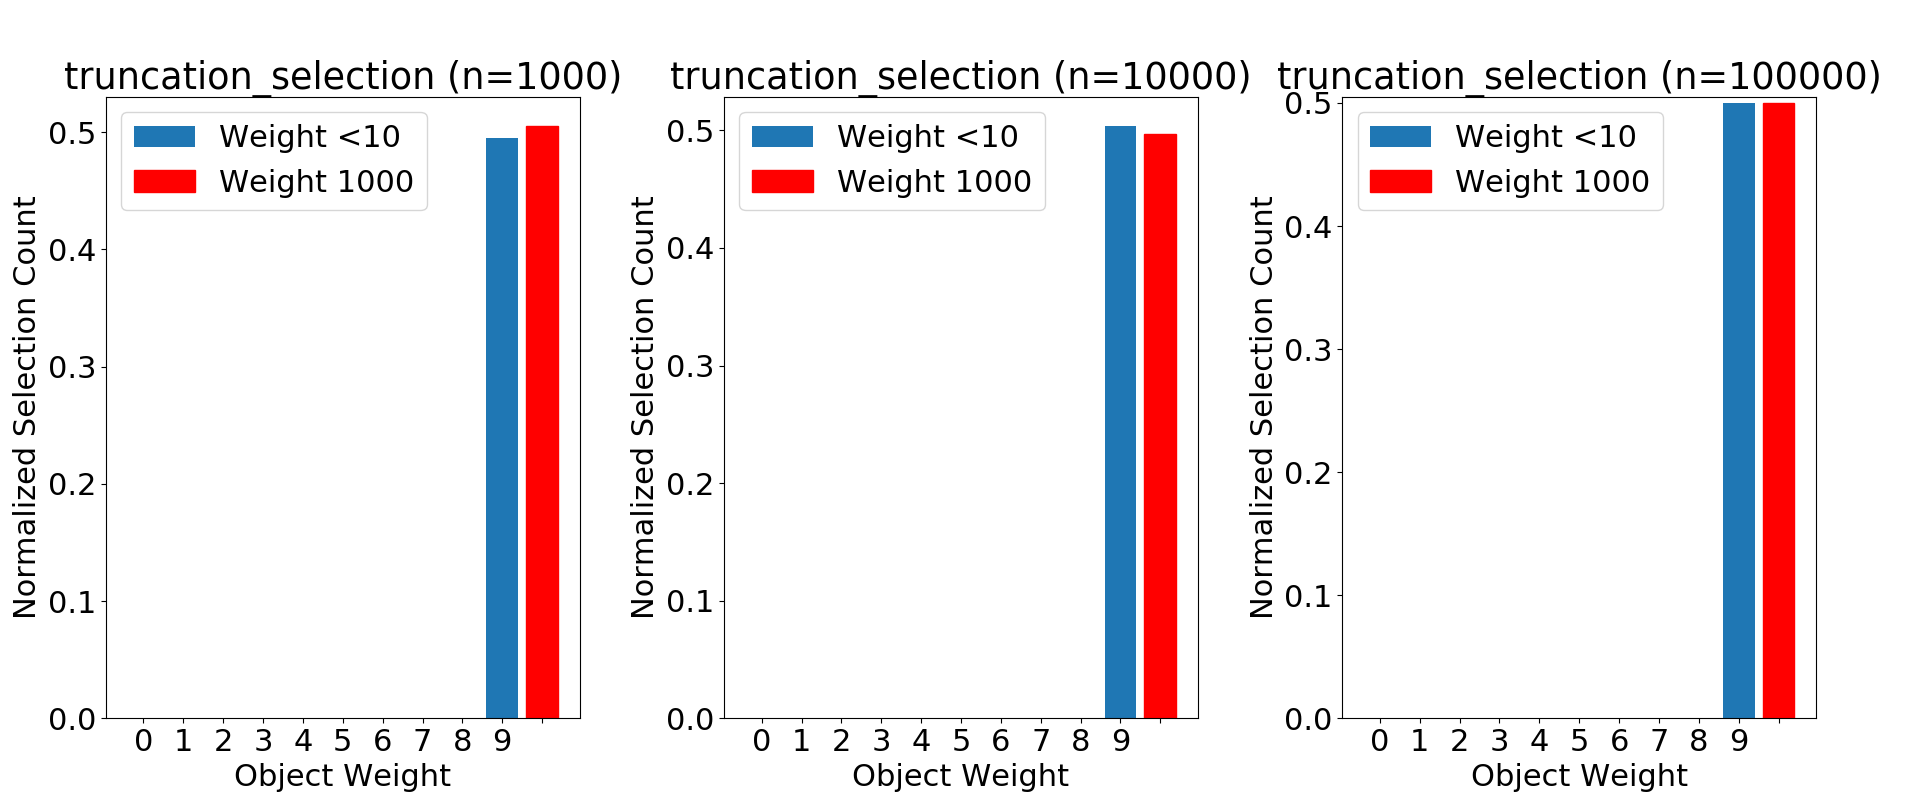
\includegraphics[scale=0.30]{images/pathological_truncation.png} 
      \caption{Histograms generated by simulation of truncation selection
               using sample sizes of 1e3, 1e4, and 1e5. Object weights are in
               the range [0,9] with a single outlier of weight 1000 to
               illustrate the effect of herding behavior.}
      \label{fig:pathological_truncation}
    \end{figure}

    \subsubsection{Two-choice Sampling Simulations}
    Two-choice sampling, first introduced by %TODO: mitzenmacher paper
    has proven to be extremely resilient to herding behavior as shown in
    Figure \ref{fig:pathological_two_choice} and selection frequencies for all
    objects are influenced by object weights in a way similar to SUS. While an
    object with a higher weight is more likely to be selected, it is not
    selected with a probability proportional to its fitness value. This makes
    the algorithm resistant to any herding behaviors, but will not be a good
    candidate if we desire the WeightedVector to select objects with
    probability proportional to its weight.

    \begin{figure}[h]
      \centering
      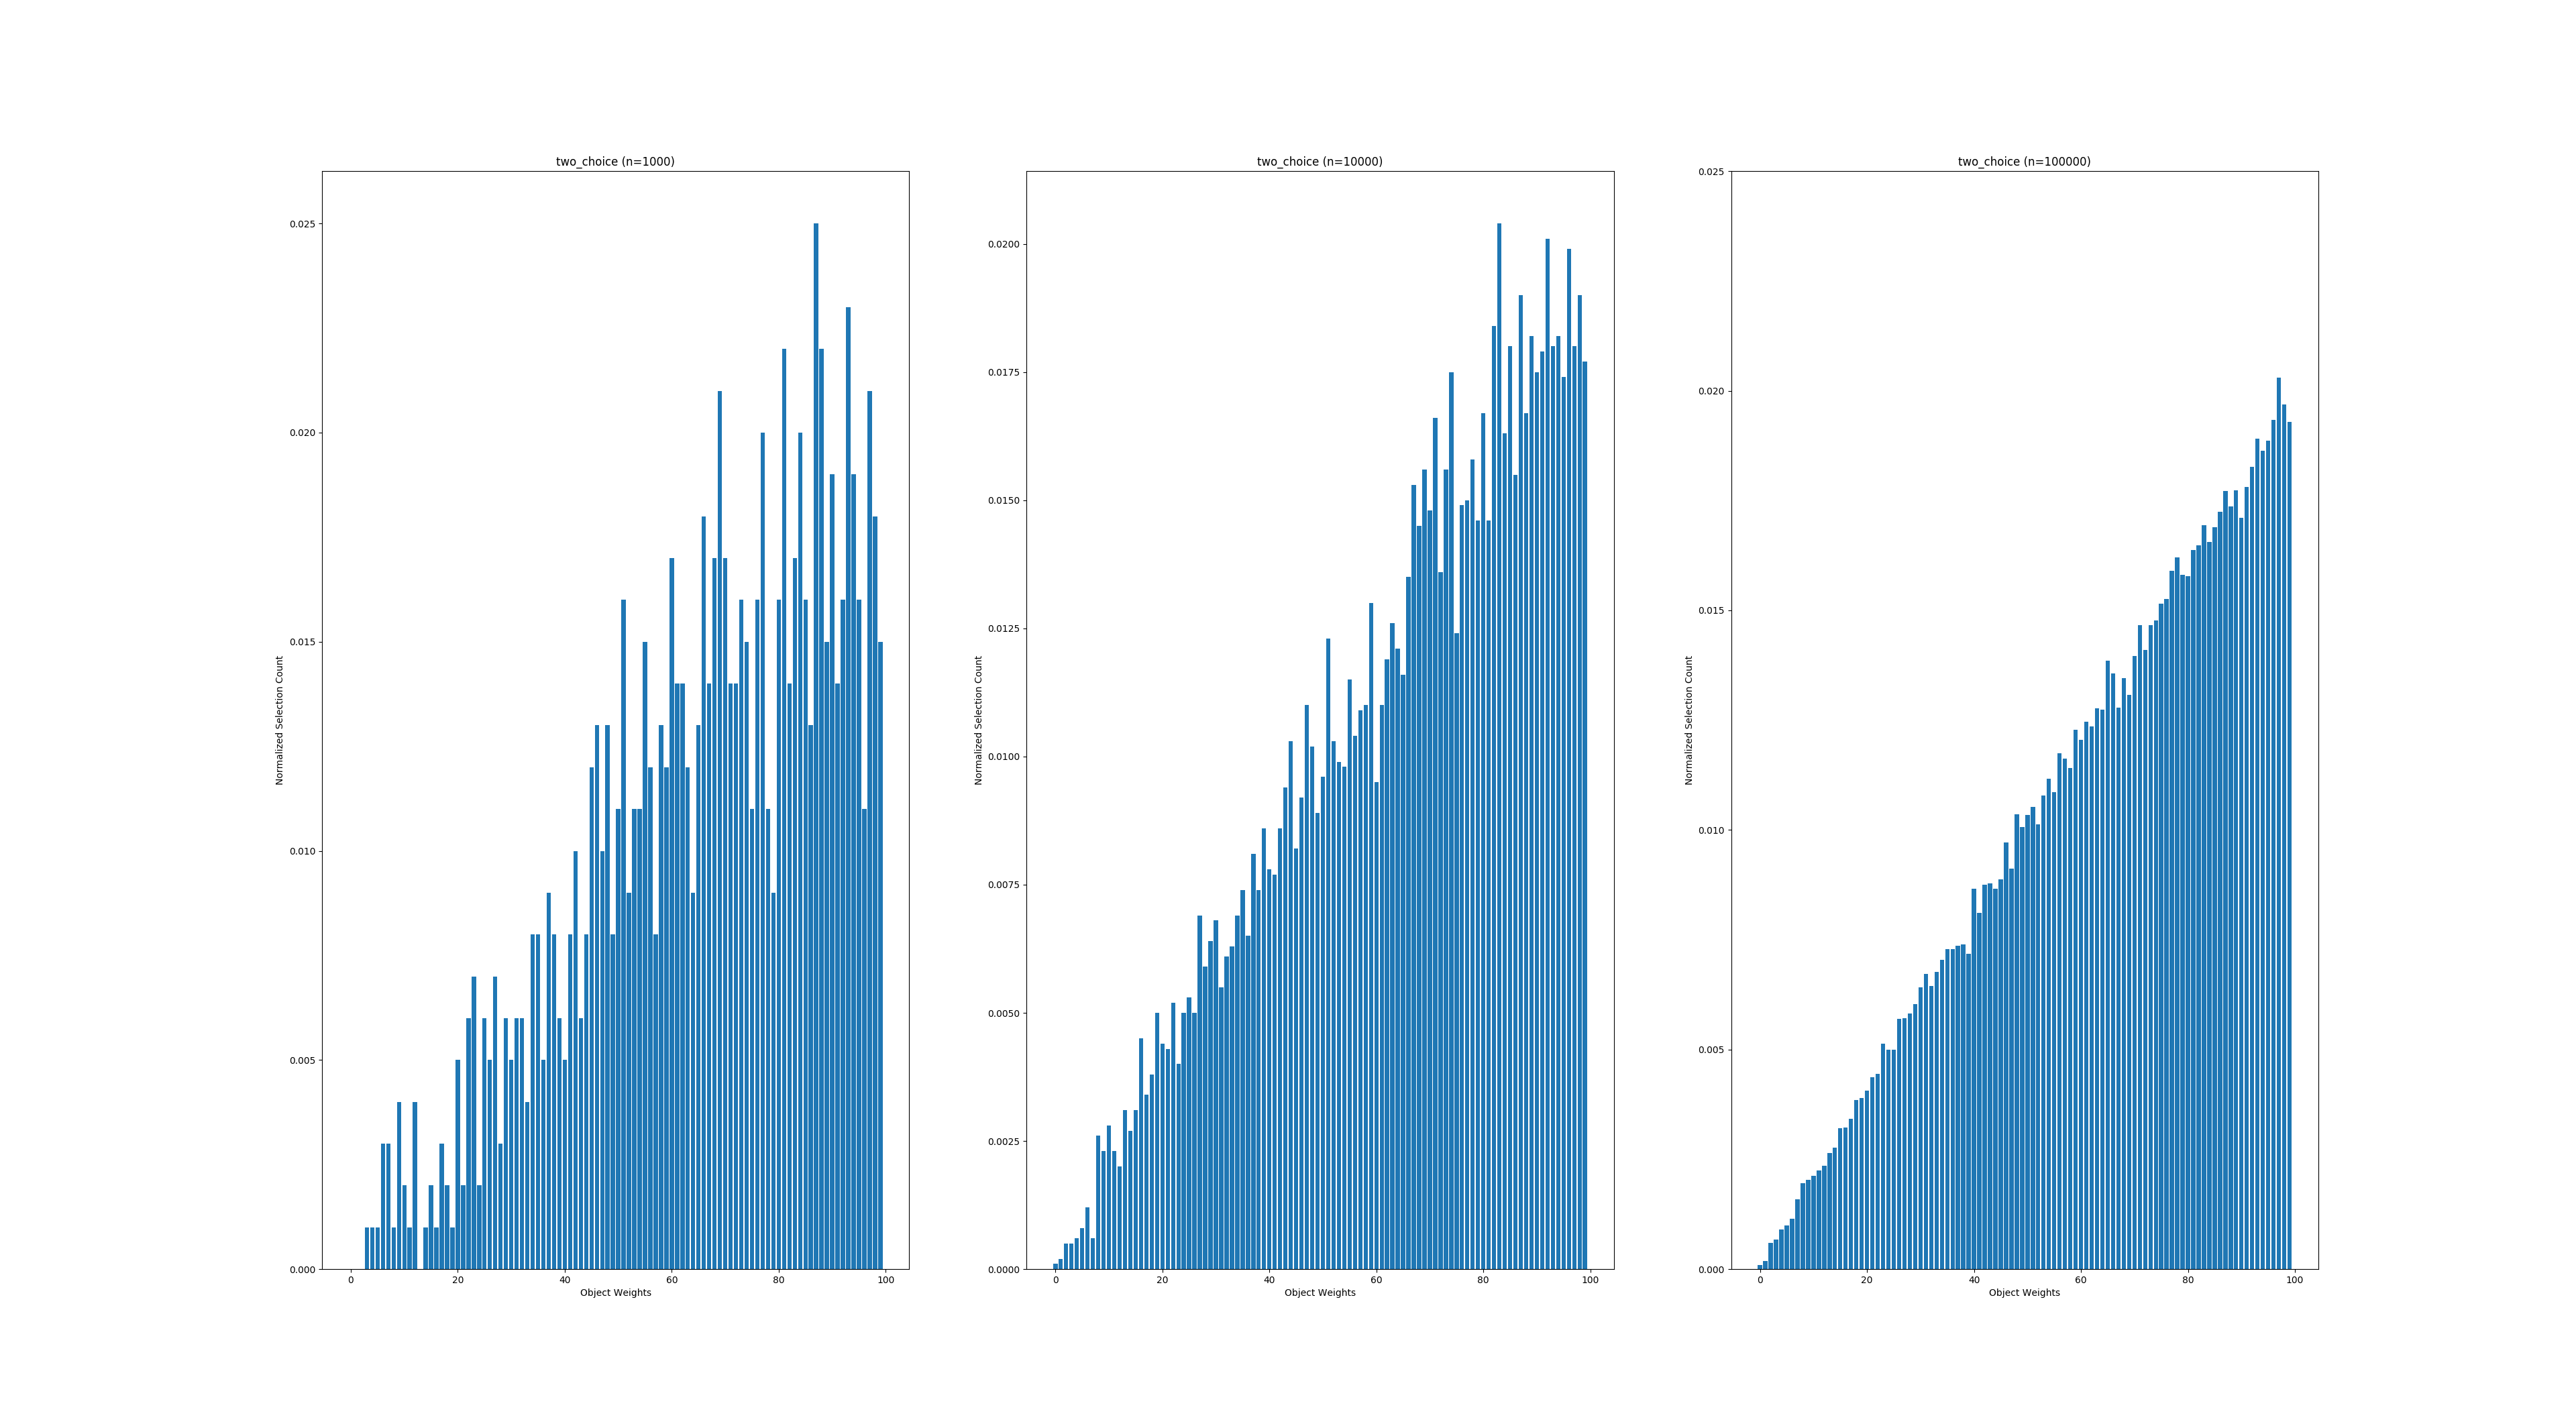
\includegraphics[scale=0.30]{images/herding_two_choice.png} 
      \caption{Histograms generated by simulation of two-choice selection
               using sample sizes of 1e3, 1e4, and 1e5. Object weights
               for the histograms are in the range [1,100].}
      \label{fig:herding_two_choice}
    \end{figure}

    \begin{figure}[h]
      \centering
      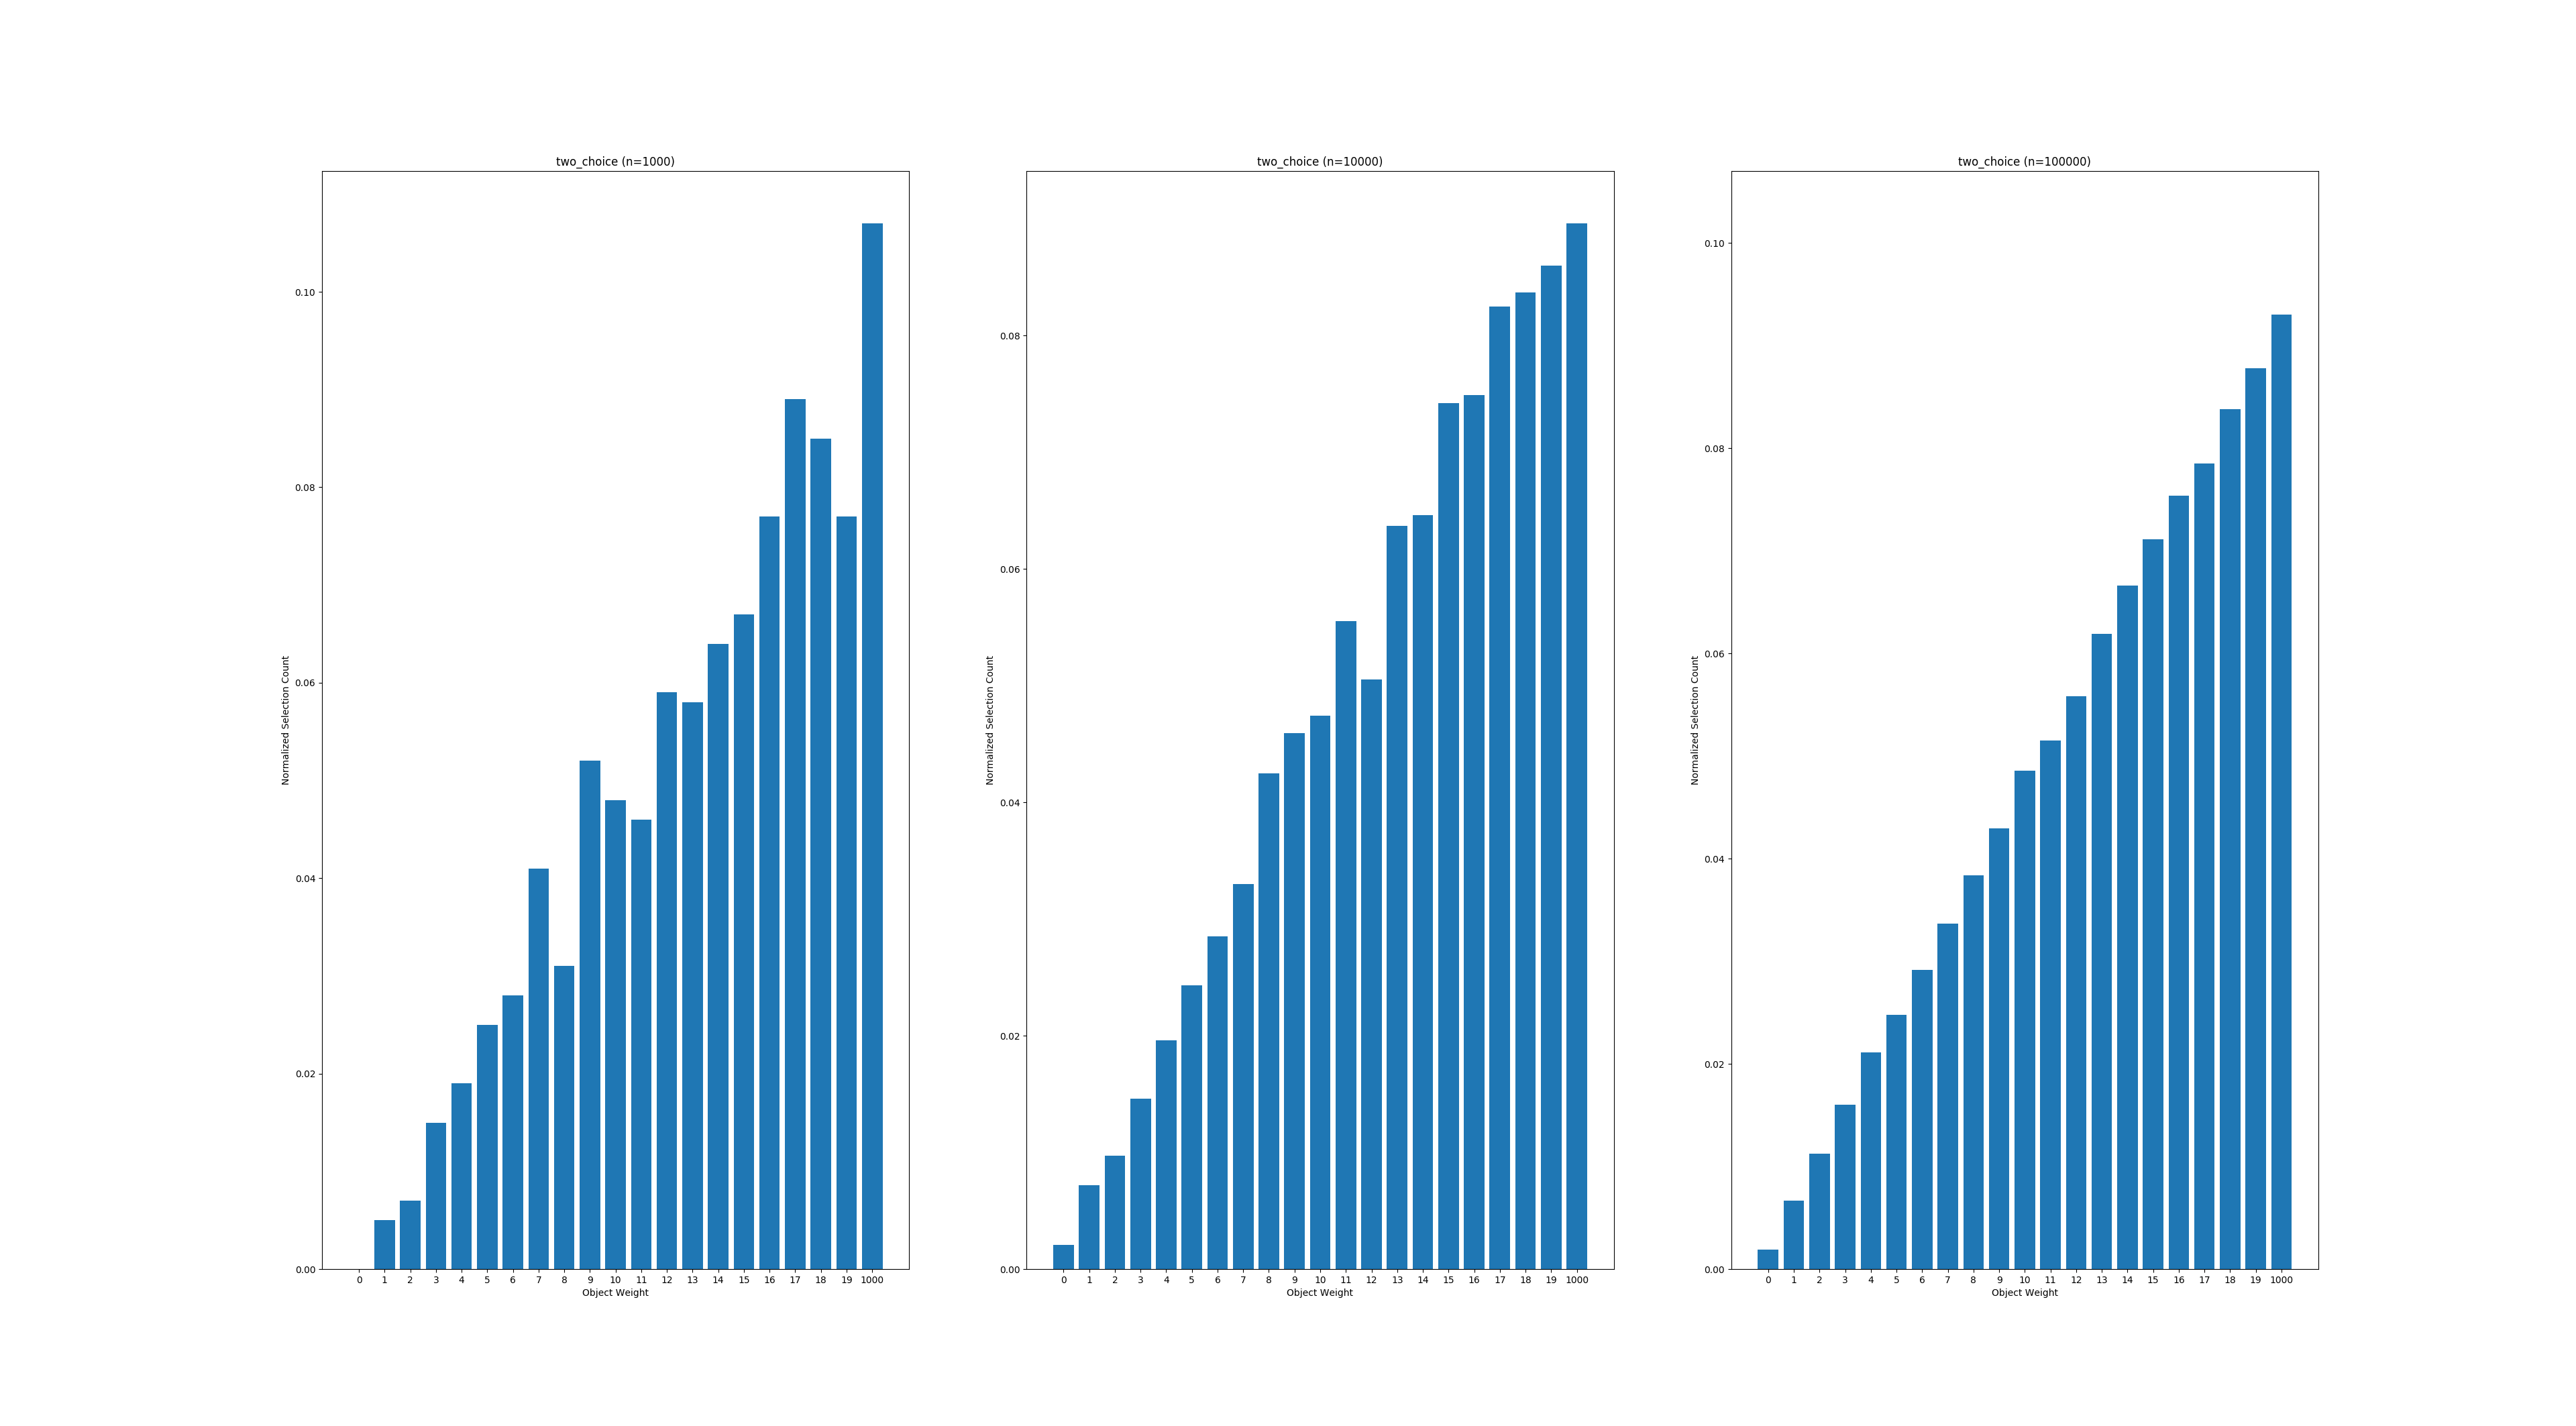
\includegraphics[scale=0.30]{images/pathological_two_choice.png} 
      \caption{Histograms generated by simulation of two-choice selection
               using sample sizes of 1e3, 1e4, and 1e5. Object weights are in
               the range [0,9] with a single outlier of weight 1000 to
               illustrate the effect of herding behavior.}
      \label{fig:pathological_two_choice}
    \end{figure}

    \subsubsection{Uniform Random Selection Simulations}
    Uniform random selection is completely indifferent to object weights.
    Therefore, it exhibits no herding behavior and no usefulness for the
    WeightedVector's sampling, but it is important to include its analysis for
    comparison with other selection algorithms.

    \begin{figure}[h]
      \centering
      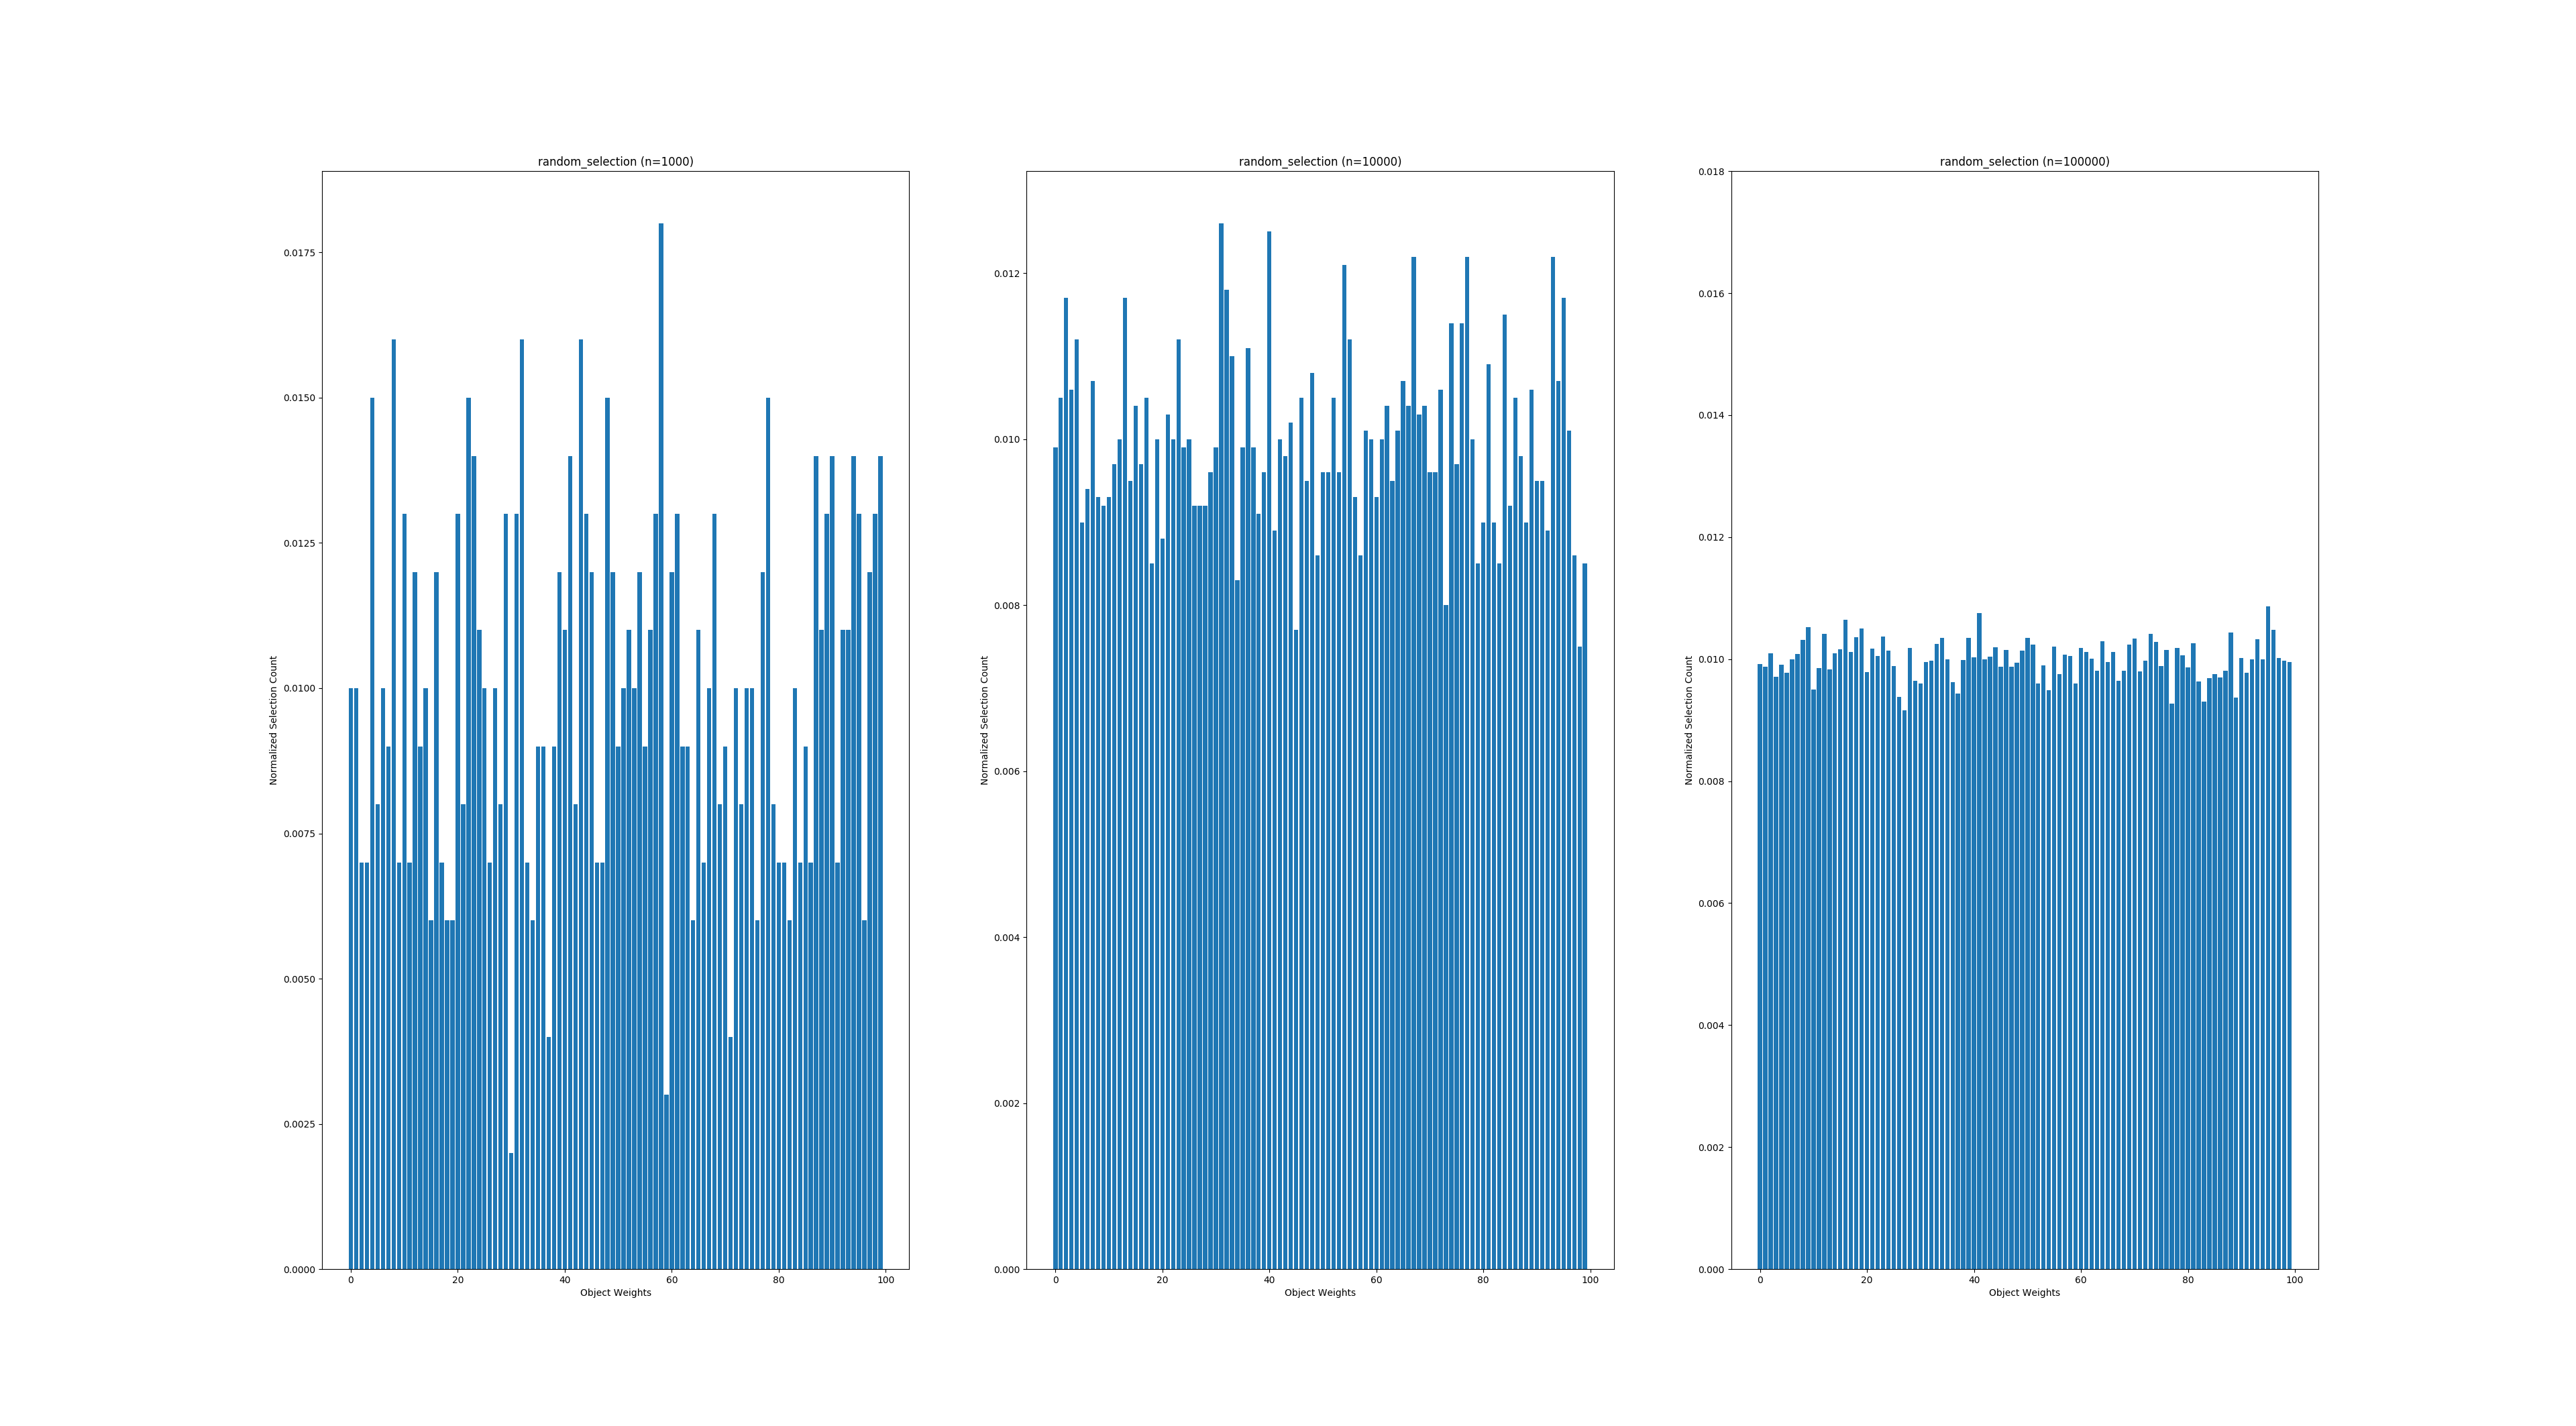
\includegraphics[scale=0.30]{images/herding_random.png} 
      \caption{Histograms generated by simulation of uniform random selection
               using sample sizes of 1e3, 1e4, and 1e5. Object weights
               for the histograms are in the range [1,100].}
      \label{fig:herding_random}
    \end{figure}

    \begin{figure}[h]
      \centering
      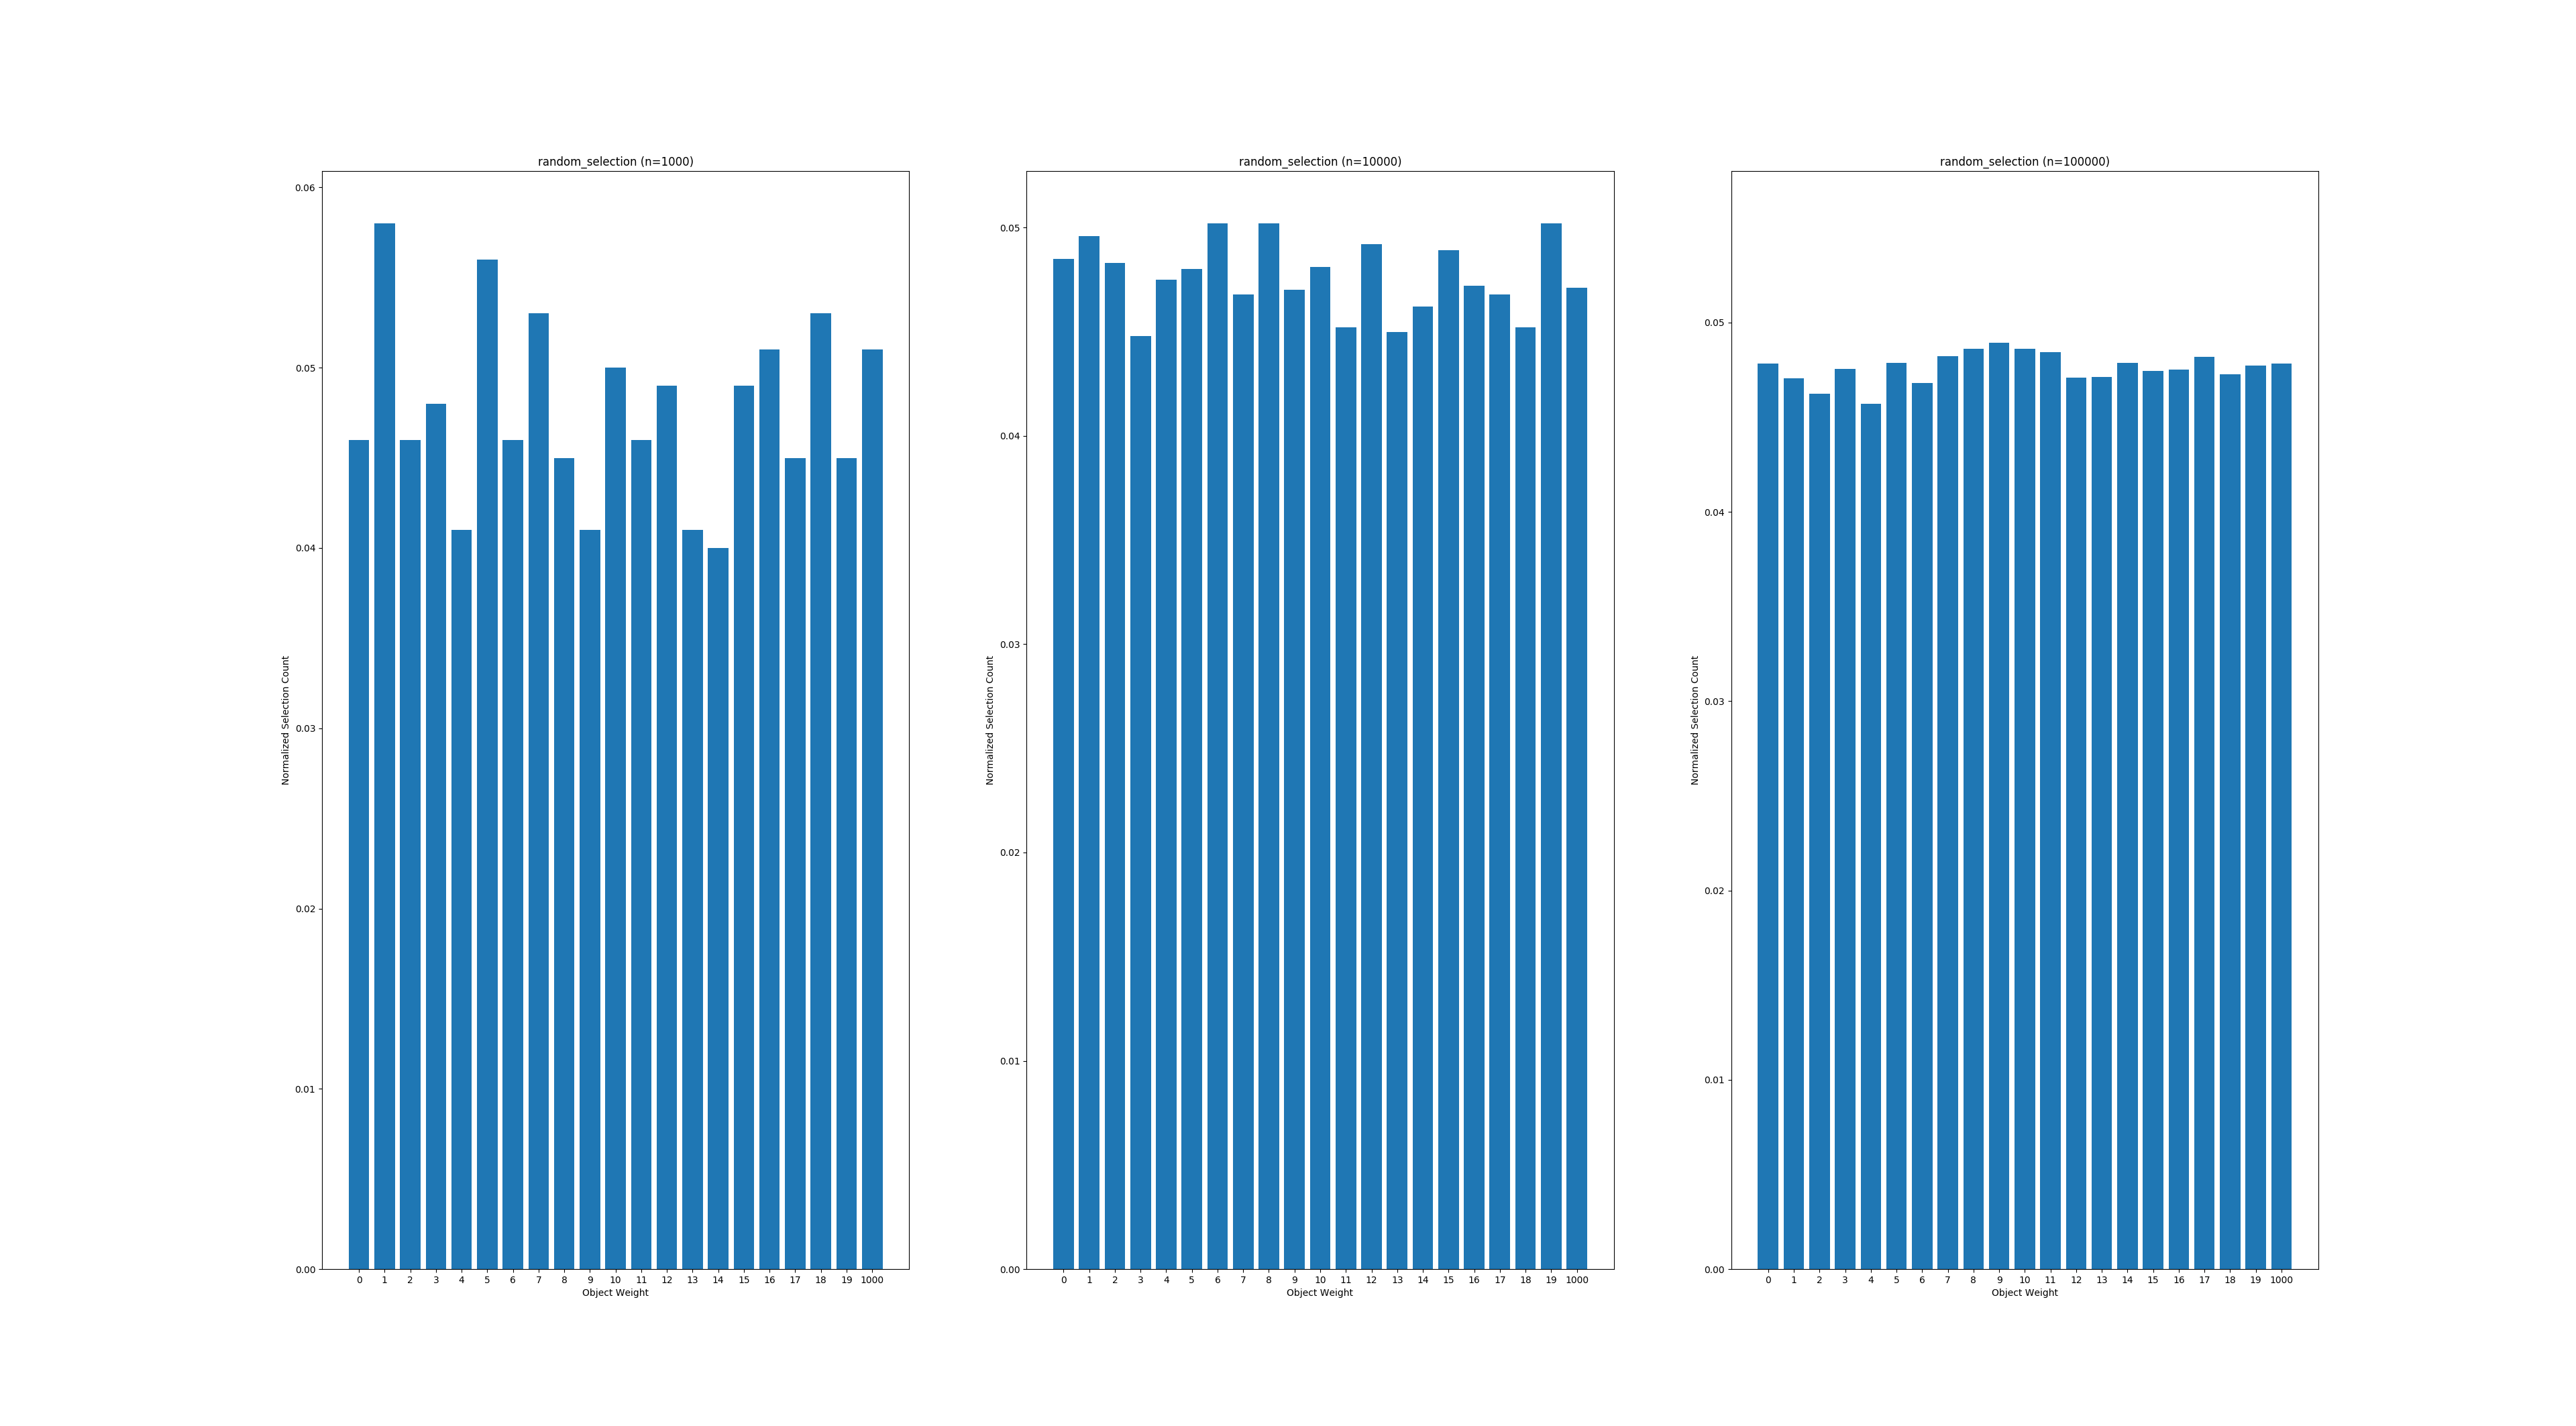
\includegraphics[scale=0.30]{images/pathological_random.png} 
      \caption{Histograms generated by simulation of uniform random selection
               using sample sizes of 1e3, 1e4, and 1e5. Object weights are in
               the range [0,9] with a single outlier of weight 1000 to
               illustrate the effect of herding behavior.}
      \label{fig:pathological_random}
    \end{figure}

    Figure \ref{fig:pathological_truncation} shows that we can expect uniform
    selection probabilities and Figure \ref{fig:pathological_random} confirms
    that we can expect no herding behavior with a uniform random selection
    scheme.

    \subsubsection{Weighted Random Algorithm Scalability Simulations}
    It's clearly seen that even though both SUS and truncation selection are
    [TODO: cite runtimes for each]
    exponential in run time, truncation selection is slower than SUS by an
    order of magnitude. This is mainly due to the need for the truncation
    selection algorithm to calculate the top T\% of the set for every selection
    performed. As expected, two-choice and random selections are
    observed to be constant-time algorithms. Two-choice is slightly slower than
    random selection due to the second selection and comparison operation that
    must occur.

    \begin{figure}[h]
      \centering
      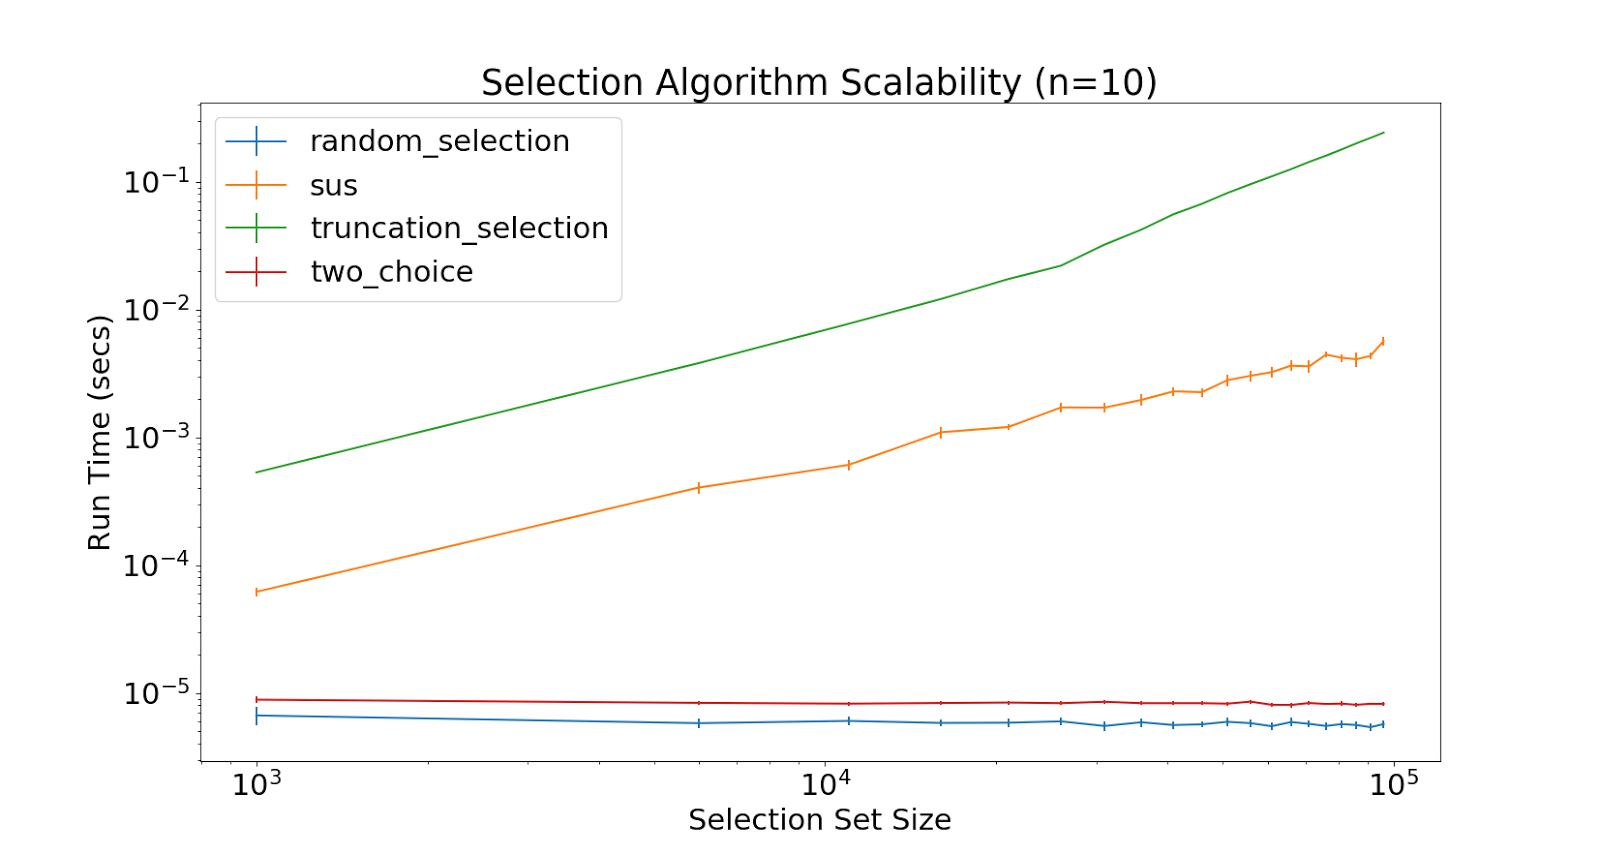
\includegraphics[scale=0.25]{images/random_scalability.png} 
      \caption{Running times of various weight random selection algorithms.
               Each algorithm is run for 10 iterations at each object pool
               size.}
      \label{fig:random_scalability}
    \end{figure}

  \subsection{WeightedVector Class}

% TODO

  \subsection{Changes to the Stargate Disk Stats}

% TODO

  \subsection{Unit Testing}

% TODO

    \subsubsection{WeightedVector Unit Tests}

% TODO

    \subsubsection{ReplicaSelector Unit Tests}

%%%%%%%%%%%%%%%%%%%%%%%%%%%%%%%%%%%%%%%%%%%%%%%%%%%%%%%%%%%%%%%%%%%%%%%%%%%%%%%
\section{Evaluation and Results}

The experiments below seek to measure the effect of the additive and
multiplicative term fitness functions on both the tier utilization of each node
and the queue lengths of disks residing on those nodes compared with uniform
random selection.

  \subsection{Experimental Setup}

  The replica selection schemes were evaluated using a NX-1350 for evaluating
  the disk fullness and a NX-3-node cluster). Each node contains a single 300GB
  SSD and 4 HDDs 1TB in size. When evaluating the new replica disk selection
  framework, two heterogeneous workload scenarios are tested:
 
  \begin{enumerate}
    \item Two worker VMs on separate nodes running a workload with low
          outstanding ops.
    \item Two worker VMs on separate nodes with running a
          workload with high outstanding ops.
  \end{enumerate}
 
  \subsection{Fio and Write Patterns}

  When generating I/O in these experiments, Fio is used on the worker VMs. Fio,
  short for Flexible IO, is an I/O workload generator that can take
  configuration files to specify the parameters of a test. On each worker VM,
  fio is used to generate a sequential write workload that completely fills the
  cluster's hot-tier. I choose to use exclusively sequential writes for all
  tests because they are the default for fio tests and the purpose of these
  experiments is to generate new replicas in a consistent manner. For the
  purposes of replica placement, the Nutanix file system does not distinguish
  targets based on the write pattern that generatred an extent group.

  \subsection{Tier Utilization Experiments}

  The tier utilization experiments define the hot-tier deviation,
  $d_{hot tier}$, as the average SSD utilization percentage of the nodes
  running a workload, $u_{w}$, subtracted by the SSD utilization percentage of
  the node without a workload, $u_{o}$:
  
  \begin{equation}
    d_{hot\ tier} = \frac{u_{w1} + u_{w2}}{u_{o}}
  \end{equation}
  
  Ideally, the idle node would absorb the majority of secondary replicas from
  the running workloads. However, uniform random selection causes only 50\% of
  secondary replicas to go to the idle node even though it can potentially
  handle more work due to the fact that it does not have to service a local
  workload. In a uniform random replica selection scheme, we expect the
  nodes running a workload have to bear 100\% of their own primary replicas and
  50\% of secondary replicas from the other worker node. This causes total SSD
  utilization to be skewed towards the worker nodes and for this skew to grow
  as the tests run. This is indicated by higher $d_{hot\ tier}$ values. We
  expect a more sophisticated replica selection scheme to minimize
  $d_{hot\ tier}$ by biasing secondary replicas towards the idle node and
  limiting the skew.

  % TODO: should I include fio scripts here, in some appendix, or in the user
  % guide?

    \subsubsection{Low Outstanding Operation Results}

    \begin{figure}[h]
      \centering
      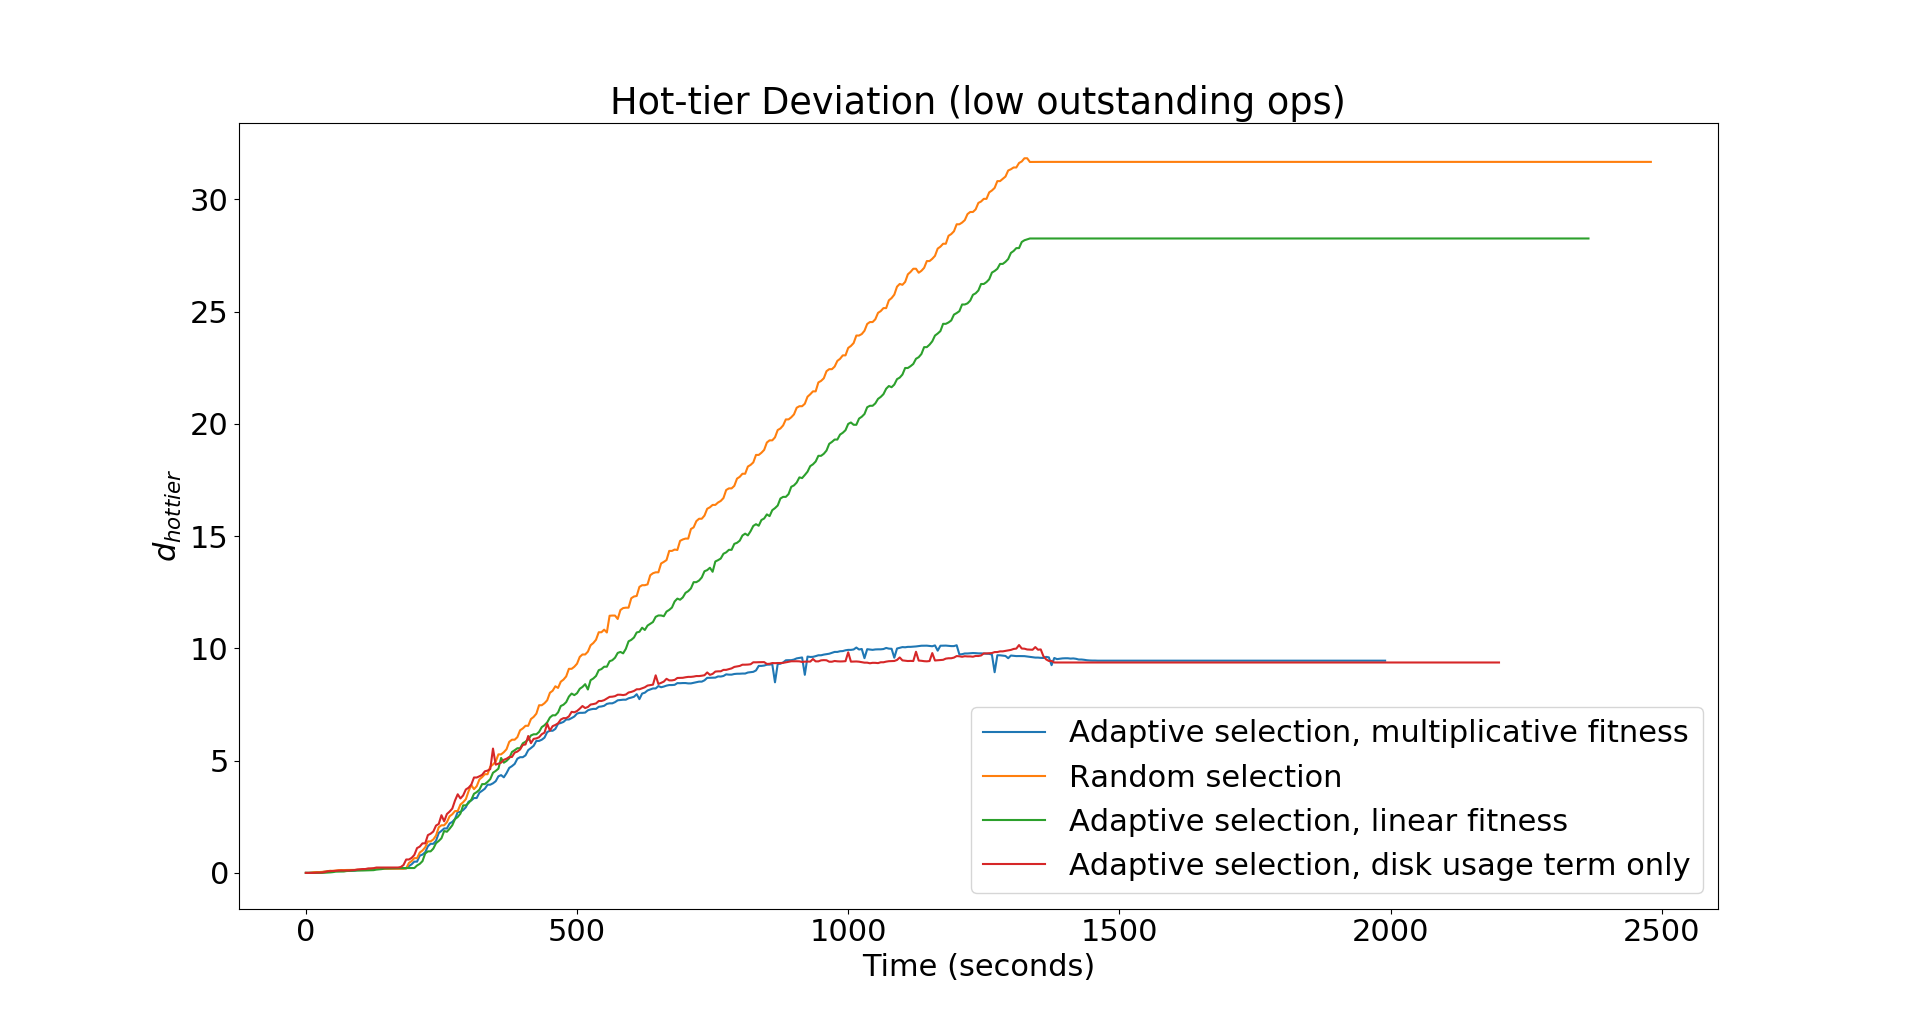
\includegraphics[scale=0.30]{images/low_outstanding_exp.png} 
      \caption{$d_{hot\ tier}$ values over time for low outstanding I/O
               operations.}
      \label{fig:low_outstanding_tier_disparity}
    \end{figure}

    Figure \ref{fig:low_outstanding_tier_disparity} shows the results of a
    workload with only a single outstanding operation. This causes the queue
    length reported by Stargate to be at most 1, resulting in the fitness
    function's queue length term to be roughly constant and approximately 1.
    
    We can see that the additive fitness function does not minimize the
    hot-tier deviation as well as the multiplicative. This is because an
    additive fitness function's behavior varies depending on the weight chosen
    for the queue length term. By default, the linear fitness function
    gives equal weight to both the disk fullness and queue length terms;
    however, for one run of this experiment the queue length term was given no
    weight. Linear fitness that gives equal weight to both terms does not
    reduce skew by very much while giving no weight to the queue length term
    keeps all nodes' usages within 10\% of each other. This is because the
    queue length term is contributing the maximum amount possible to the
    fitness value due to the consistently low queue length values. We can
    illustrate this by defining a disk selection bias, $b_r$, as the
    probability some disk, $d$, will be selected when compared with another
    disk, $d'$ whose utilization is 10\% higher and queue length value is
    identical. Given a fitness function, $f$, we can calculate $b_r$ as
    follows:

    \begin{equation}
      b_r = \frac{f(d)}{f(d) + f(d')}
    \end{equation}

    Figures \ref{fig:bias_max_qlen} and \ref{fig:bias_min_qlen} show the disk
    selection biases for very large and very small queue lengths respectively.

    \begin{figure}[h]
      \centering
      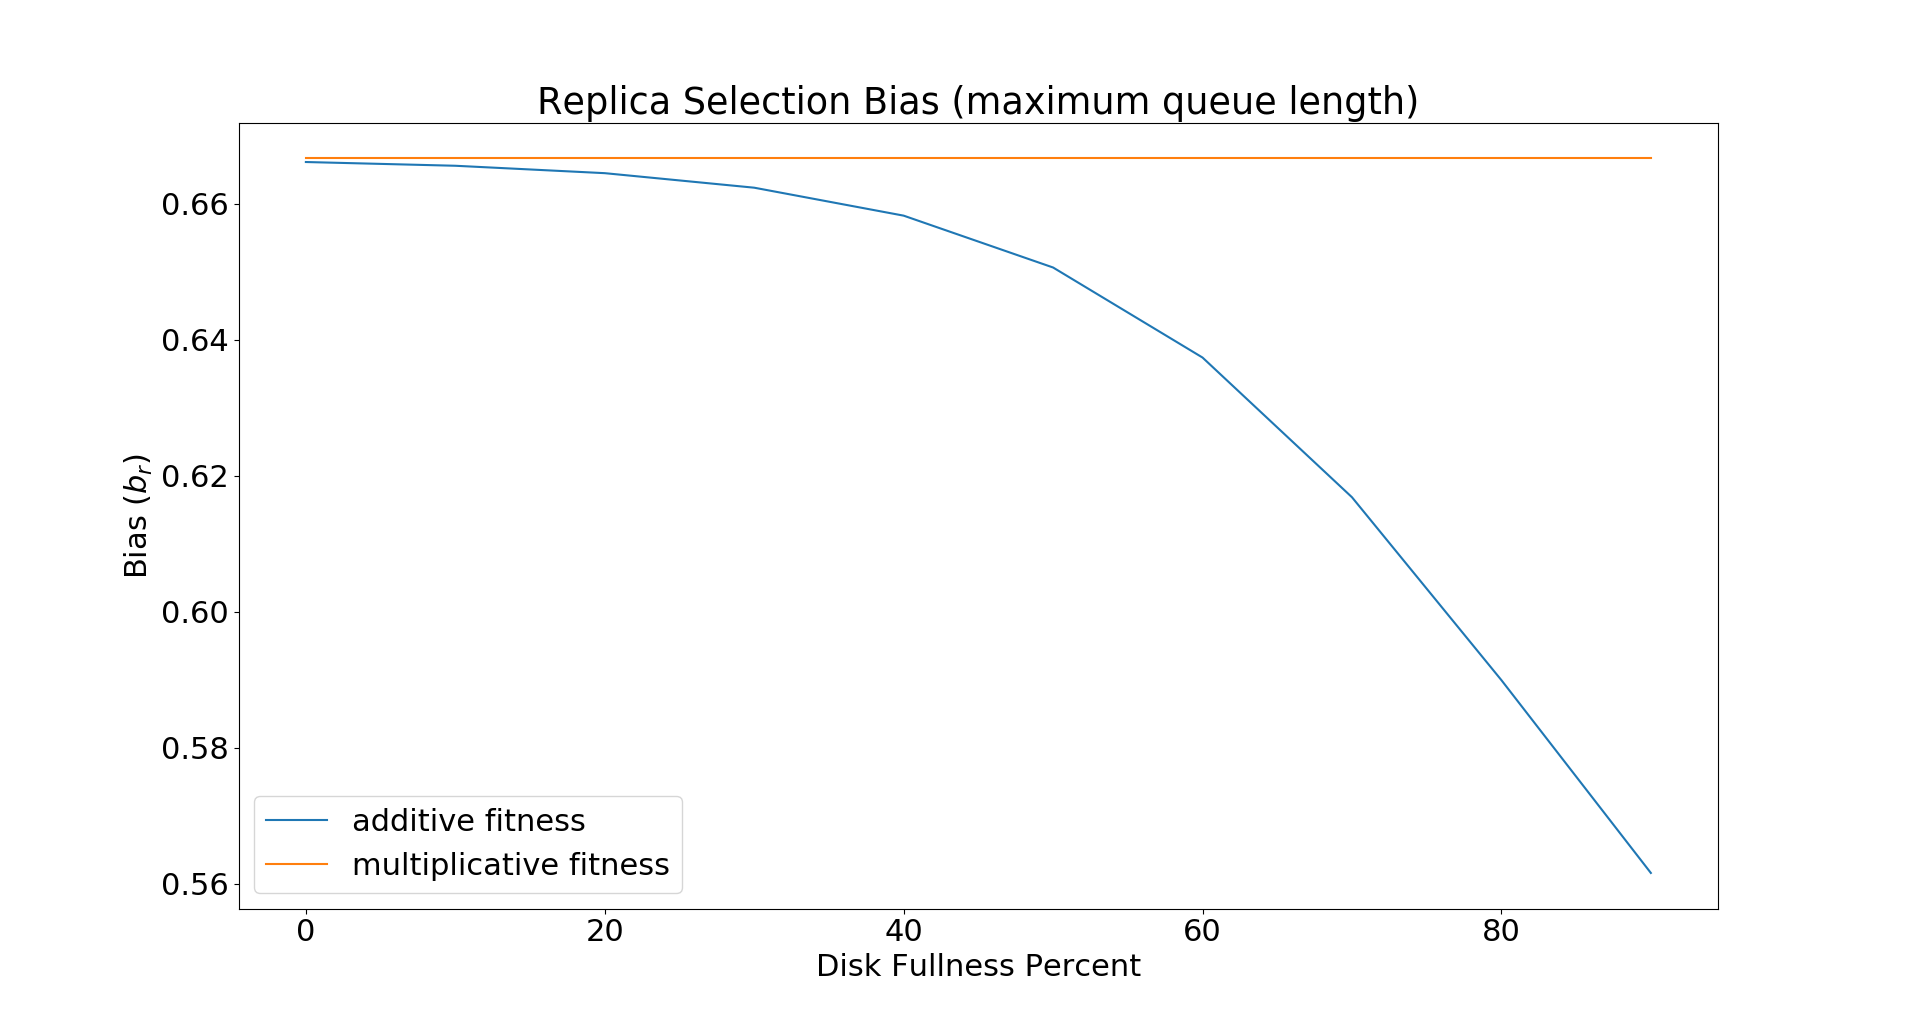
\includegraphics[scale=0.30]{images/replica_selection_bias_max_qlen.png} 
      \caption{$b_r$ values with static queue lengths at the fitness
               function ceiling values.}
      \label{fig:bias_max_qlen}
    \end{figure}

    \begin{figure}[h]
      \centering
      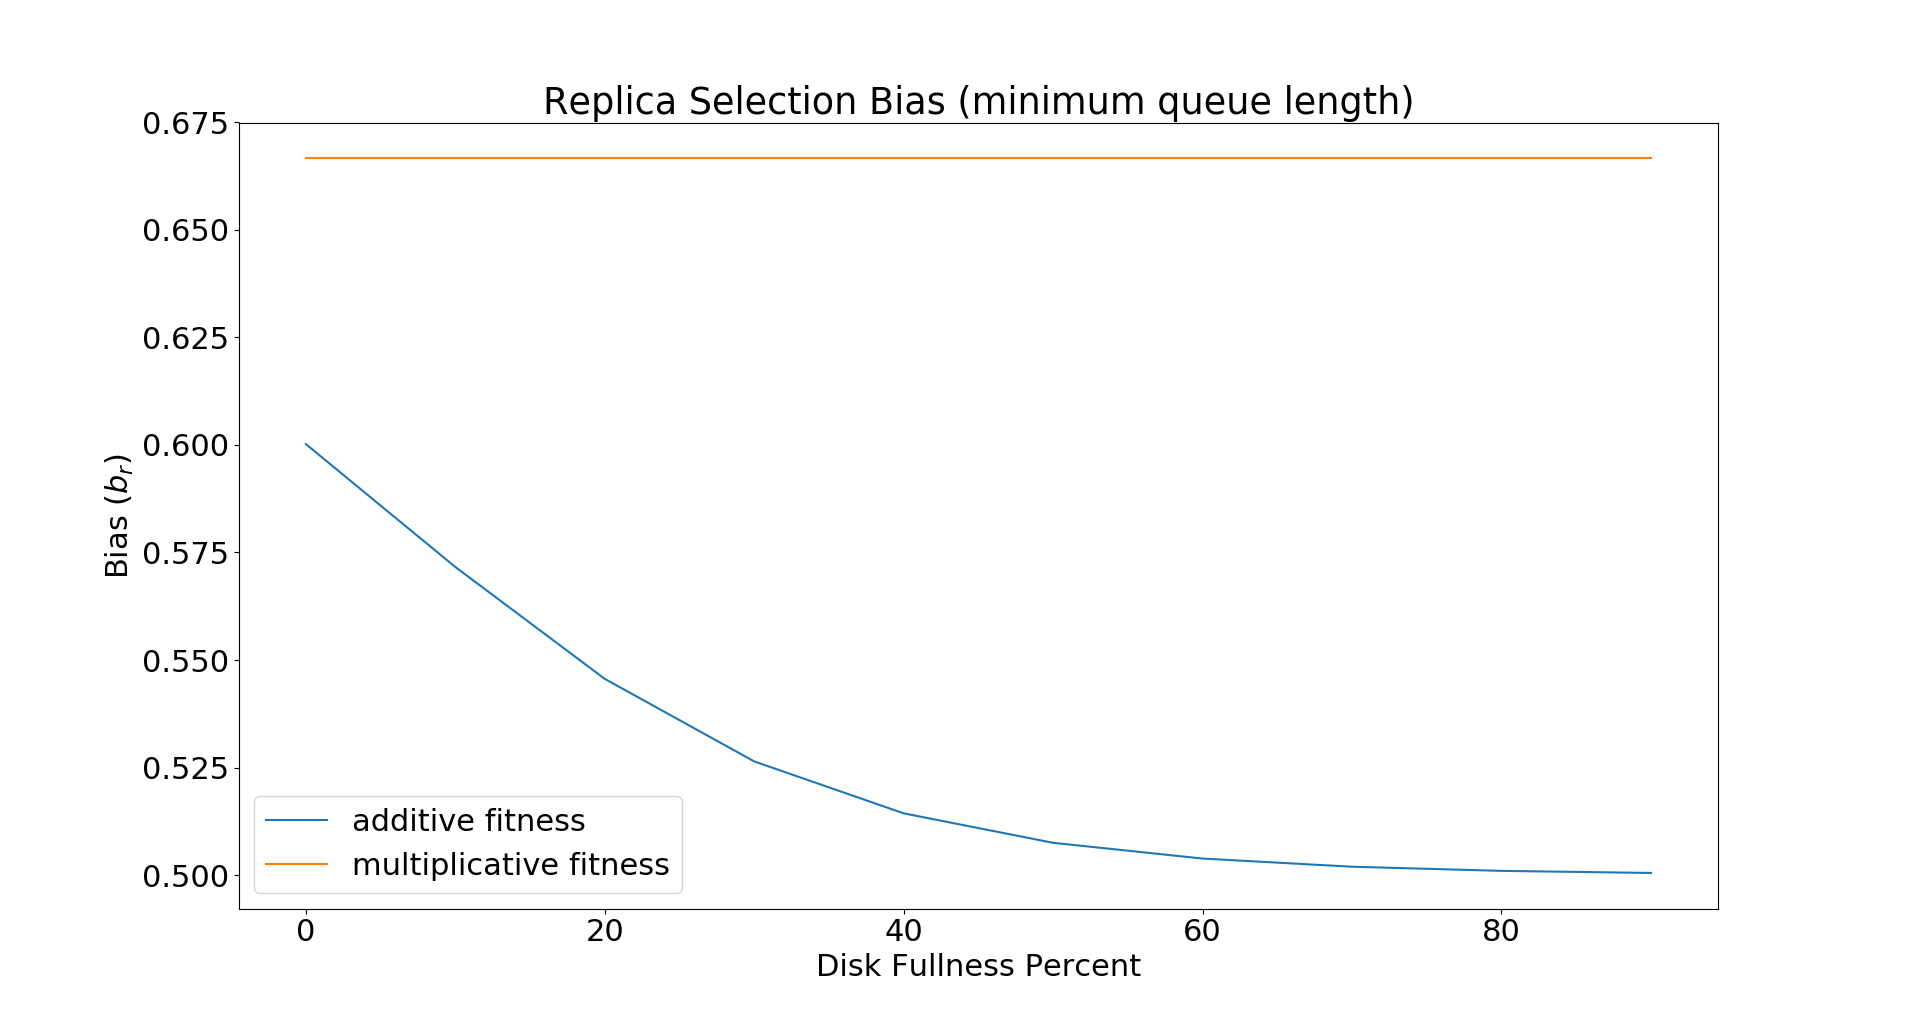
\includegraphics[scale=0.30]{images/replica_selection_bias_min_qlen.png} 
      \caption{$b_r$ values with static queue lengths at 1.}
      \label{fig:bias_min_qlen}
    \end{figure}

    We can see that for an additive fitness function, the bias towards a less
    utilized disk decreases as the disk fullness percentages for $d$ and $d'$
    increase, even though they still only differ by 10\% in the figure above.
    This is because the entire linear fitness function does not scale with each
    term, so we can conclude that the multiplicative fitness function is
    superior.

    \subsubsection{High Outstanding Operation Results}

    \begin{figure}[h]
      \centering
      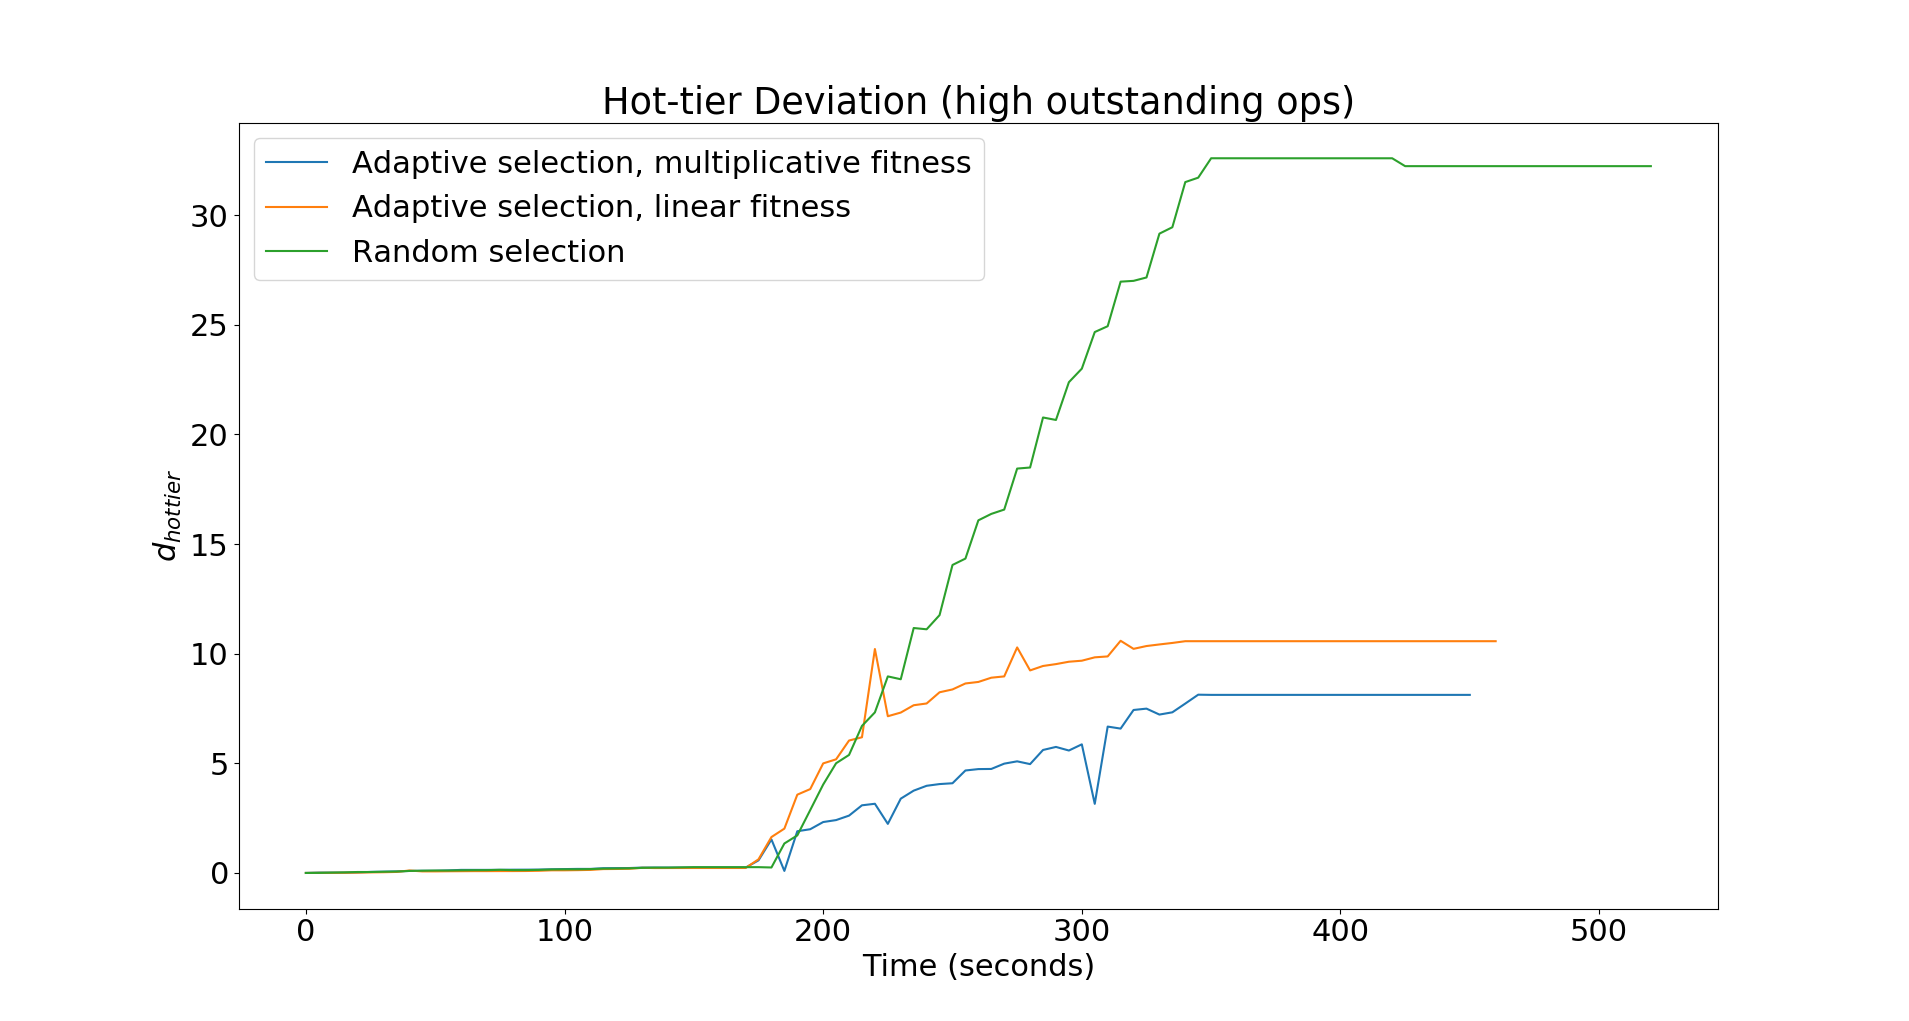
\includegraphics[scale=0.30]{images/high_outstanding_exp.png} 
      \caption{$d_{hot\ tier}$ values over time for low outstanding I/O
               operations.}
      \label{fig:high_outstanding_tier_disparity}
    \end{figure}


    In Figure \ref{fig:high_outstanding_tier_disparity}, we can see that both
    additive and multiplicative fitness functions reduce the disk fullness skew
    from 30\% to less than 10\%. Multiplicative fitness performs slightly
    better at minimizing $d_{hot\ tier}$ than additive fitness, possibly due to
    scaling the fitness value by the value of both the fullness and queue
    length terms, rather than weights.
  
  \subsection{Disk Queue Length Experiments}

  Since a low outstanding operation workload would not give useful
  information for measuring the effects of fitness-based replica selection on
  disk queue lengths, the high outstanding I/O operation experiment in the
  previous section was re-run for all fitness function types and for fitness
  function queue length term ceilings of 200 and 100. Figures
  \ref{fig:qlen_100} and \ref{fig:qlen_200} show a reduction in
  queue length quartiles when fitness-based selection is used for disks on
  nodes that host local workloads. Lower queue length ceilings are
  observed to provide better results in reducing the queue lengths for the
  worker nodes.

  \begin{figure}[!htb]
    \centering
    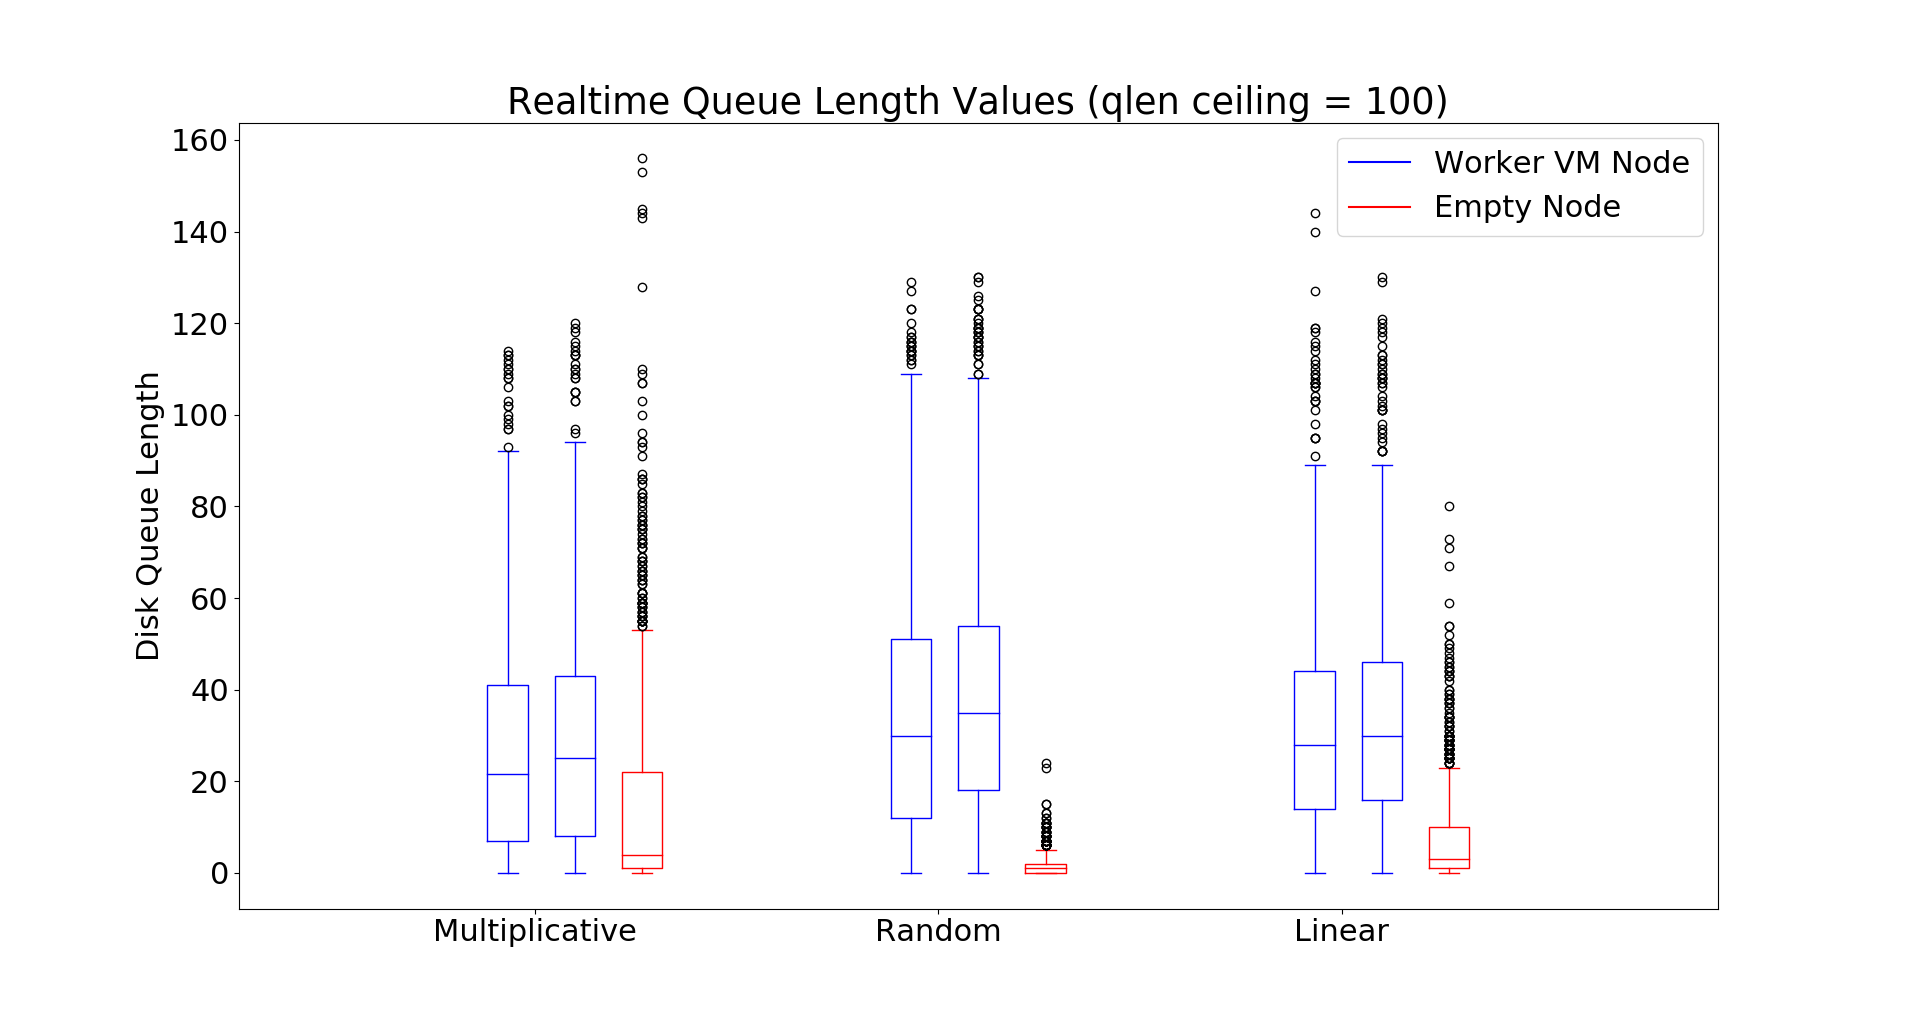
\includegraphics[scale=0.30]{images/qlen_100_box.png} 
    \caption{Queue lengths for all SSDs on the specified nodes sampled every 1
             second.}
    \label{fig:qlen_100}
  \end{figure}

  \begin{figure}[!htb]
    \centering
    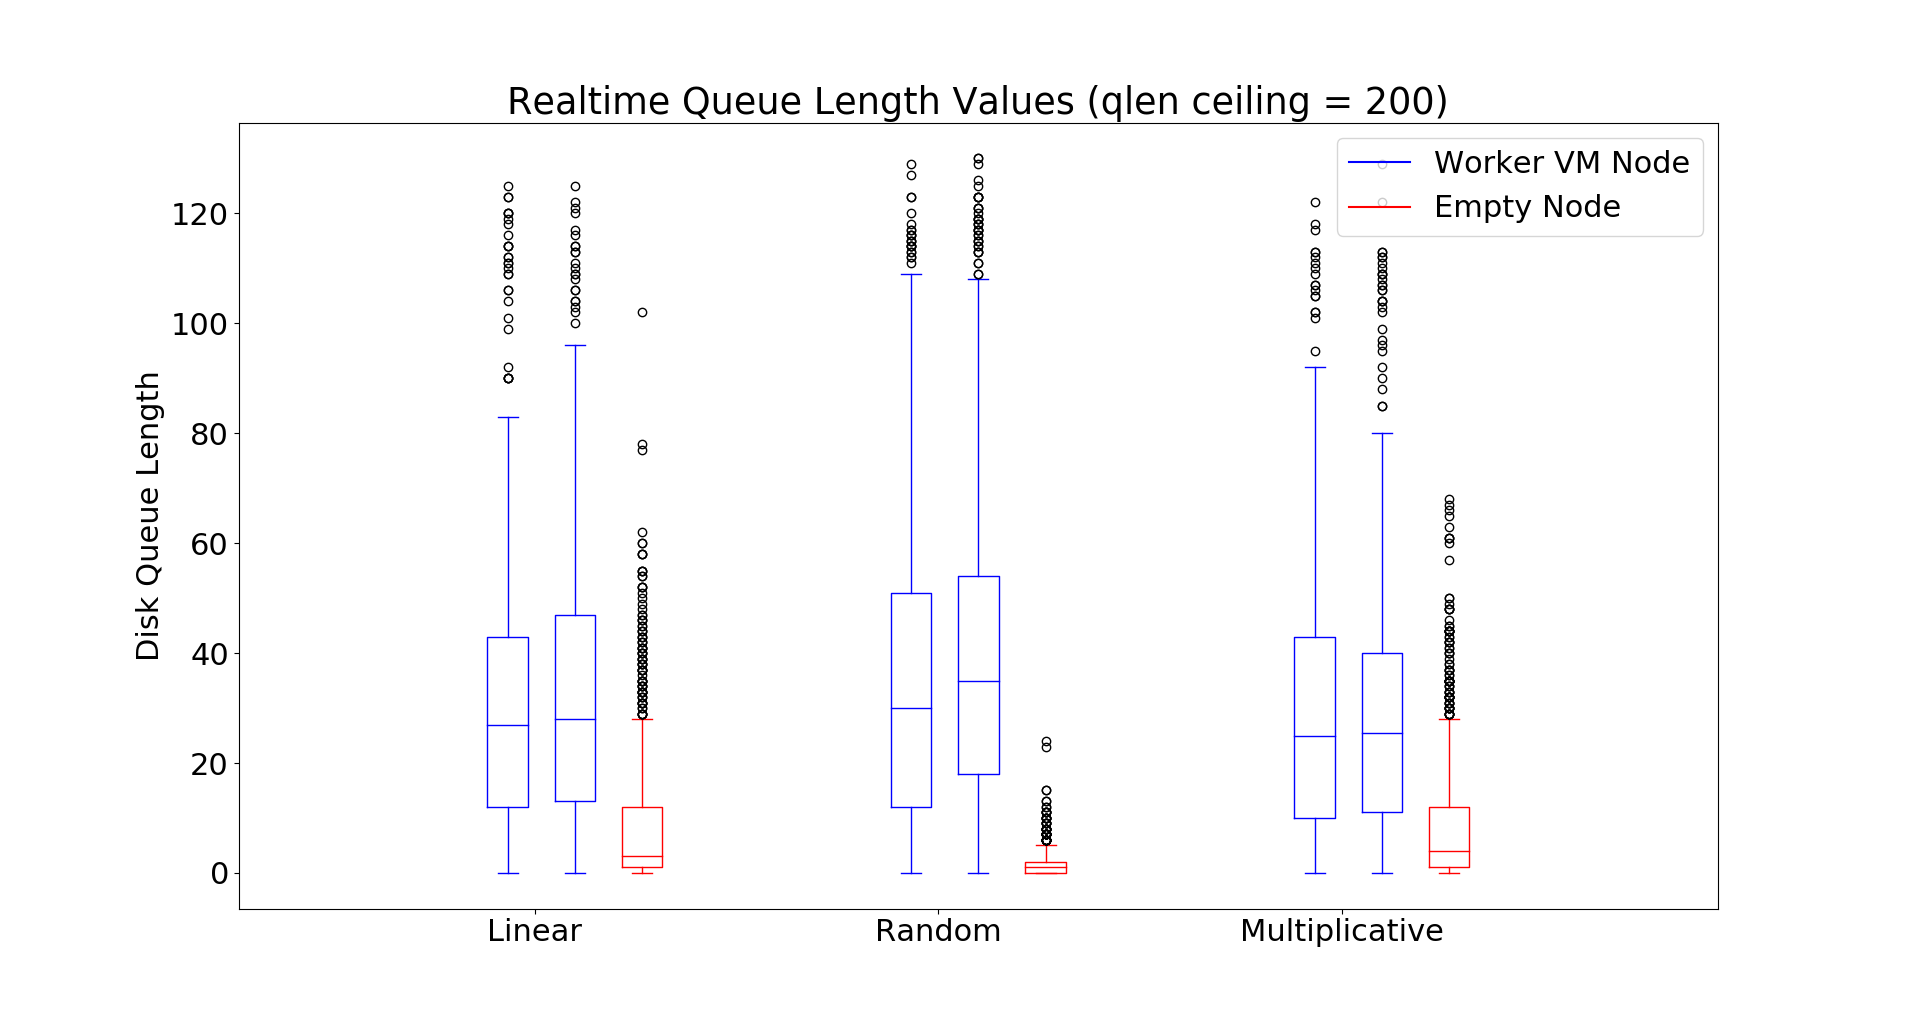
\includegraphics[scale=0.30]{images/qlen_200_box.png} 
    \caption{Queue lengths for all SSDs on the specified nodes sampled every 1
             second.}
    \label{fig:qlen_200}
  \end{figure}

%%%%%%%%%%%%%%%%%%%%%%%%%%%%%%%%%%%%%%%%%%%%%%%%%%%%%%%%%%%%%%%%%%%%%%%%%%%%%%%
\section{User Guide}

% TODO

  \subsection{Re-creating Experiments}

% TODO

  \subsection{Scraping Data From the Nutanix Cluster}

%%%%%%%%%%%%%%%%%%%%%%%%%%%%%%%%%%%%%%%%%%%%%%%%%%%%%%%%%%%%%%%%%%%%%%%%%%%%%%%
\section{Conclusions}

% TODO

  \subsection{Summary}

% TODO

    \subsubsection{Low Outstanding Operation Test}

% TODO

    \subsubsection{High Outstanding Operation Test}

  \subsection{Conclusion}

    % Explain how this work solves the stated problems.

% TODO

  \subsection{Future Work}

% TODO

    \subsubsection{Real-time Fitness Feedback}

      % Realtime feedback from disks using historical latency numbers.
    
% TODO

    \subsubsection{Read Replica Selection}

      % Based on historical latencies.

% TODO

    \subsubsection{More Fitness Function Variables}

      % CPU, disk wear, data access patterns.

% TODO

%%%%%%%%%%%%%%%%%%%%%%%%%%%%%%%%%%%%%%%%%%%%%%%%%%%%%%%%%%%%%%%%%%%%%%%%%%%%%%%
\section{Appendix}

% TODO

  \subsection{Herding Behavior Due to Implementation Bug}

% TODO

  \subsection{Glossary}

% TODO

  \subsection{References}

% TODO


\end{document}
